%===============================================================================
% LaTeX sjabloon voor de bachelorproef toegepaste informatica aan HOGENT
% Meer info op https://github.com/HoGentTIN/latex-hogent-report
%===============================================================================

\documentclass[dutch,dit,thesis]{hogentreport}

\usepackage{lipsum} % For blind text, can be removed after adding actual content

%% Pictures to include in the text can be put in the graphics/ folder
\graphicspath{{graphics/}}

%% For source code highlighting, requires pygments to be installed
%% Compile with the -shell-escape flag!
\usepackage[section]{minted}
%% If you compile with the make_thesis.{bat,sh} script, use the following
%% import instead:
%% \usepackage[section,outputdir=../output]{minted}
\usemintedstyle{solarized-light}
\definecolor{bg}{RGB}{253,246,227} %% Set the background color of the codeframe

%% Change this line to edit the line numbering style:
\renewcommand{\theFancyVerbLine}{\ttfamily\scriptsize\arabic{FancyVerbLine}}

%% Macro definition to load external java source files with \javacode{filename}:
\newmintedfile[javacode]{java}{
    bgcolor=bg,
    fontfamily=tt,
    linenos=true,
    numberblanklines=true,
    numbersep=5pt,
    gobble=0,
    framesep=2mm,
    funcnamehighlighting=true,
    tabsize=4,
    obeytabs=false,
    breaklines=true,
    mathescape=false
    samepage=false,
    showspaces=false,
    showtabs =false,
    texcl=false,
}

% Other packages not already included can be imported here

%%---------- Document metadata -------------------------------------------------
\author{Sarah Eggermont}
\supervisor{Dhr. S. Labijn}
\cosupervisor{Dhr. G. Vande Maele}
\title[Een proof of concept]%
    {Competitief sportplatform met gamification zodat werknemers in een sedentaire job meer bewegen}
\academicyear{\advance\year by -1 \the\year--\advance\year by 1 \the\year}
\examperiod{1}
\degreesought{\IfLanguageName{dutch}{Professionele bachelor in de toegepaste informatica}{Bachelor of applied computer science}}
\partialthesis{false} %% To display 'in partial fulfilment'
%\institution{Internshipcompany BVBA.}

%% Add global exceptions to the hyphenation here
\hyphenation{back-slash}

%% The bibliography (style and settings are  found in hogentthesis.cls)
\addbibresource{bachproef.bib}            %% Bibliography file
\addbibresource{../voorstel/voorstel.bib} %% Bibliography research proposal
\defbibheading{bibempty}{}

%% Prevent empty pages for right-handed chapter starts in twoside mode
\renewcommand{\cleardoublepage}{\clearpage}

\renewcommand{\arraystretch}{1.2}

%% Content starts here.
\begin{document}

%---------- Front matter -------------------------------------------------------

\frontmatter

\hypersetup{pageanchor=false} %% Disable page numbering references
%% Render a Dutch outer title page if the main language is English
\IfLanguageName{english}{%
    %% If necessary, information can be changed here
    \degreesought{Professionele Bachelor toegepaste informatica}%
    \begin{otherlanguage}{dutch}%
       \maketitle%
    \end{otherlanguage}%
}{}

%% Generates title page content
\maketitle
\hypersetup{pageanchor=true}

%%=============================================================================
%% Voorwoord
%%=============================================================================

\chapter*{\IfLanguageName{dutch}{Woord vooraf}{Preface}}%
\label{ch:voorwoord}

%% TODO:
%% Het voorwoord is het enige deel van de bachelorproef waar je vanuit je
%% eigen standpunt (``ik-vorm'') mag schrijven. Je kan hier bv. motiveren
%% waarom jij het onderwerp wil bespreken.
%% Vergeet ook niet te bedanken wie je geholpen/gesteund/... heeft

TODO
%%=============================================================================
%% Samenvatting
%%=============================================================================

% TODO: De "abstract" of samenvatting is een kernachtige (~ 1 blz. voor een thesis) synthese van het document.
%
% Een goede abstract biedt een kernachtig antwoord op volgende vragen:
%
% 1. Waarover gaat de bachelorproef?
% 2. Waarom heb je er over geschreven?
% 3. Hoe heb je het onderzoek uitgevoerd?
% 4. Wat waren de resultaten? Wat blijkt uit je onderzoek?
% 5. Wat betekenen je resultaten? Wat is de relevantie voor het werkveld?
%
% Daarom bestaat een abstract uit volgende componenten:
%
% - inleiding + kaderen thema
% - probleemstelling
% - (centrale) onderzoeksvraag
% - onderzoeksdoelstelling
% - methodologie
% - resultaten (beperk tot de belangrijkste, relevant voor de onderzoeksvraag)
% - conclusies, aanbevelingen, beperkingen



%%---------- Samenvatting -----------------------------------------------------
% De samenvatting in de hoofdtaal van het document

\chapter*{\IfLanguageName{dutch}{Samenvatting}{Abstract}}

Beweging speelt een grote rol in zowel de fysieke als de mentale gezondheid van mensen. Bijna één derde van de wereldbevolking beweegt te weinig en ondervindt hier vroeg of laat de nadelen van. Om die reden bespreekt dit onderzoek of een sportplatform, dat gebruik maakt van gamification, gebruikt kan worden om medewerkers van \href{https://en.joule.be/}{Joule}, \href{https://www.ventures4growth.com/en}{Ventures 4 Growth}, \href{https://www.mace-legal.com/}{mace}, \href{https://planetb.life/en}{PlanetB}, \href{https://www.we-are.be/}{we are} en \href{https://www.delaware.pro/en-be}{delaware}, die een sedentaire job beoefenen, aan te zetten om meer te sporten.

Na een literatuurstudie rond het belang van beweging, gamification en hoe gamification de intrinsieke motivatie om te bewegen kan bevorderen, worden werknemers van eerder genoemde bedrijven geïnterviewd om de succescriteria en de benodigdheden van het nieuwe platform te bepalen. Aan de hand van deze criteria wordt een platform, in de vorm van een responsive website, gecreëerd. In deze proof of concept wordt gamification geïmplementeerd en worden sportgegevens van deelnemende werknemers verzameld en grafisch voorgesteld op het platform. Tegelijkertijd wordt ook de beleving omtrent het gamification-aspect bevraagd. Deze gegevens leiden, samen met de eerder verzamelde data, tot de conclusie van dit onderzoek.

Dit onderzoek suggereert dat een sportplatform met gamification wel degelijk zorgt voor een verbetering in de hoeveelheid beweging van mensen in een sedentaire job. Daarnaast stelt het dat gamificationtechnieken zoals punten en scoreborden, vooral wanneer dit zorgt voor een onderlinge competitie, het meest succesvol zijn. Tenslotte zijn er in dit onderzoek geen gamificationtechnieken opgemerkt die een negatief effect hebben op de hoeveelheid beweging van gebruikers, maar moet wel opgemerkt worden dat, binnen de context van een sportapplicatie, personen het storend vinden om meldingen te ontvangen als deel van de gamification.

%---------- Inhoud, lijst figuren, ... -----------------------------------------

\tableofcontents

% In a list of figures, the complete caption will be included. To prevent this,
% ALWAYS add a short description in the caption!
%
%  \caption[short description]{elaborate description}
%
% If you do, only the short description will be used in the list of figures

\listoffigures

% If you included tables and/or source code listings, uncomment the appropriate
% lines.
%\listoftables
%\listoflistings

% Als je een lijst van afkortingen of termen wil toevoegen, dan hoort die
% hier thuis. Gebruik bijvoorbeeld de ``glossaries'' package.
% https://www.overleaf.com/learn/latex/Glossaries

%---------- Kern ---------------------------------------------------------------

\mainmatter{}

% De eerste hoofdstukken van een bachelorproef zijn meestal een inleiding op
% het onderwerp, literatuurstudie en verantwoording methodologie.
% Aarzel niet om een meer beschrijvende titel aan deze hoofdstukken te geven of
% om bijvoorbeeld de inleiding en/of stand van zaken over meerdere hoofdstukken
% te verspreiden!

%%=============================================================================
%% Inleiding
%%=============================================================================

\chapter{\IfLanguageName{dutch}{Inleiding}{Introduction}}%
\label{ch:inleiding}

%\begin{itemize}
%  \item context, achtergrond
%  \item afbakenen van het onderwerp
%  \item verantwoording van het onderwerp, methodologie
%  \item probleemstelling
%  \item onderzoeksdoelstelling
%  \item onderzoeksvraag
%  \item \ldots
%\end{itemize}

\section{\IfLanguageName{dutch}{Probleemstelling}{Problem Statement}}%
\label{sec:probleemstelling}

Een sedentaire job wordt geassocieerd met schadelijke gevolgen voor de algemene gezondheid \autocite{Buckley2015}. Het is daarom van groot belang dat voldoende beweging een prioriteit is.

\textcite{Hallal2012} beschouwen 31,1\% van de wereldwijde bevolking als inactief. Dit wil zeggen dat, op het moment van dit onderzoek, bijna een derde van de volwassen wereldbevolking de vooropgestelde aanbevelingen van de ``World Health Organization'' (WHO), beschreven door \textcite{Bull2020}, niet haalt. Voor Europa ligt deze waarde zelfs op 34,8\% \autocite{Bull2020}.

Concreet zal deze paper bij (een deel van de) werknemers van \href{https://en.joule.be/}{Joule}, \href{https://www.ventures4growth.com/en}{Ventures 4 Growth}, \href{https://www.mace-legal.com/}{mace}, \href{https://planetb.life/en}{PlanetB}, \href{https://www.we-are.be/}{we are} en \href{https://www.delaware.pro/en-be}{delaware}, die allen een sedentaire job beoefenen, onderzoeken hoe het huidige beweeggedrag is, en of een competitief sportplatform hen kan helpen de vooropgestelde hoeveelheden van de WHO te behalen. Er zijn namelijk reeds verschillende onderzoeken, zoals de paper van \textcite{Kari2016}, die bewezen dat sportplatformen met spelelementen kunnen leiden tot een verhoogde bewegingsmotivatie, maar \textcite{Hamari2013a} kaartte aan dat dit gewenste effect zeker niet voor iedereen van toepassing is. Daarom zal dit onderzoek zich specifiek richten op personen met een sedentaire job, daar \textcite{Vandelanotte2015} geen bewijs vonden dat zij in hun vrije tijd meer bewegen om het gebrek aan beweging tijdens hun job te compenseren, wat het belang van het stimuleren van de bewegingsmotivatie verhoogt.

%Uit je probleemstelling moet duidelijk zijn dat je onderzoek een meerwaarde heeft voor een concrete doelgroep. De doelgroep moet goed gedefinieerd en afgelijnd zijn. Doelgroepen als ``bedrijven,'' ``KMO's'', systeembeheerders, enz.~zijn nog te vaag. Als je een lijstje kan maken van de personen/organisaties die een meerwaarde zullen vinden in deze bachelorproef (dit is eigenlijk je steekproefkader), dan is dat een indicatie dat de doelgroep goed gedefinieerd is. Dit kan een enkel bedrijf zijn of zelfs één persoon (je co-promotor/opdrachtgever).

\section{\IfLanguageName{dutch}{Onderzoeksvraag}{Research question}}%
\label{sec:onderzoeksvraag}

%Wees zo concreet mogelijk bij het formuleren van je onderzoeksvraag. Een onderzoeksvraag is trouwens iets waar nog niemand op dit moment een antwoord heeft (voor zover je kan nagaan). Het opzoeken van bestaande informatie (bv. ``welke tools bestaan er voor deze toepassing?'') is dus geen onderzoeksvraag. Je kan de onderzoeksvraag verder specifiëren in deelvragen. Bv.~als je onderzoek gaat over performantiemetingen, dan

Deze paper zal de volgende onderzoeksvragen beantwoorden: heeft het competitief
sportplatform, dat gebruik maakt van gamification, een positieve invloed
op het sportgedrag van werknemers in een sedentaire job? Welke gamificationtechnieken
hebben het meeste succes? Zijn er technieken die een negatief effect
hebben?

\section{\IfLanguageName{dutch}{Onderzoeksdoelstelling}{Research objective}}%
\label{sec:onderzoeksdoelstelling}

Om de problematiek uit de probleemstelling te proberen verhelpen, zal een sportplatform ontwikkeld worden. Deze ``Proof Of Concept'' (POC) zal het onderzoek faciliteren naar hoe gamification mensen in een sedentaire job kan helpen meer te bewegen in hun dagelijks leven. Gamification is in de literatuur beschreven als het gebruiken van spelelementen die niet aan een spel gerelateerd zijn \autocite{Gaalen2020}. Het gebruik van deze elementen zorgt voor een bepaalde competitie.

%Wat is het beoogde resultaat van je bachelorproef? Wat zijn de criteria voor succes? Beschrijf die zo concreet mogelijk. Gaat het bv.\ om een proof-of-concept, een prototype, een verslag met aanbevelingen, een vergelijkende studie, enz.

\section{\IfLanguageName{dutch}{Opzet van deze bachelorproef}{Structure of this bachelor thesis}}%
\label{sec:opzet-bachelorproef}

De rest van deze bachelorproef is als volgt opgebouwd:

In Hoofdstuk~\ref{ch:stand-van-zaken} wordt een overzicht gegeven van de stand van zaken binnen het onderzoeksdomein, op basis van een literatuurstudie.

In Hoofdstuk~\ref{ch:methodologie} wordt de methodologie toegelicht en worden de gebruikte onderzoekstechnieken besproken om een antwoord te kunnen formuleren op de onderzoeksvragen.

In Hoofdstuk~\ref{ch:proofofconcept} worden de gekozen technologieën van de POC toegelicht en wordt de opbouw van de applicatie besproken.

In Hoofdstuk~\ref{ch:analyse} worden de cijfers geanalyseerd die uit zowel de bevragingen als de website komen.

In Hoofdstuk~\ref{ch:conclusie}, tenslotte, wordt de conclusie gegeven en een antwoord geformuleerd op de onderzoeksvragen. Daarbij wordt ook een aanzet gegeven voor toekomstig onderzoek binnen dit domein.
\chapter{\IfLanguageName{dutch}{Stand van zaken}{State of the art}}%
\label{ch:stand-van-zaken}

% Tip: Begin elk hoofdstuk met een paragraaf inleiding die beschrijft hoe
% dit hoofdstuk past binnen het geheel van de bachelorproef. Geef in het
% bijzonder aan wat de link is met het vorige en volgende hoofdstuk.

% Pas na deze inleidende paragraaf komt de eerste sectiehoofding.

% Dit hoofdstuk bevat je literatuurstudie. De inhoud gaat verder op de inleiding, maar zal het onderwerp van de bachelorproef *diepgaand* uitspitten. De bedoeling is dat de lezer na lezing van dit hoofdstuk helemaal op de hoogte is van de huidige stand van zaken (state-of-the-art) in het onderzoeksdomein. Iemand die niet vertrouwd is met het onderwerp, weet nu voldoende om de rest van het verhaal te kunnen volgen, zonder dat die er nog andere informatie moet over opzoeken \autocite{Pollefliet2011}.

% Je verwijst bij elke bewering die je doet, vakterm die je introduceert, enz.\ naar je bronnen. In \LaTeX{} kan dat met het commando \texttt{$\backslash${textcite\{\}}} of \texttt{$\backslash${autocite\{\}}}. Als argument van het commando geef je de ``sleutel'' van een ``record'' in een bibliografische databank in het Bib\LaTeX{}-formaat (een tekstbestand). Als je expliciet naar de auteur verwijst in de zin (narratieve referentie), gebruik je \texttt{$\backslash${}textcite\{\}}. Soms is de auteursnaam niet expliciet een onderdeel van de zin, dan gebruik je \texttt{$\backslash${}autocite\{\}} (referentie tussen haakjes). Dit gebruik je bv.~bij een citaat, of om in het bijschrift van een overgenomen afbeelding, broncode, tabel, enz. te verwijzen naar de bron. In de volgende paragraaf een voorbeeld van elk.

% \textcite{Knuth1998} schreef een van de standaardwerken over sorteer- en zoekalgoritmen. Experten zijn het erover eens dat cloud computing een interessante opportuniteit vormen, zowel voor gebruikers als voor dienstverleners op vlak van informatietechnologie~\autocite{Creeger2009}.

% Let er ook op: het \texttt{cite}-commando voor de punt, dus binnen de zin. Je verwijst meteen naar een bron in de eerste zin die erop gebaseerd is, dus niet pas op het einde van een paragraaf.

Deze paragraaf beschrijft de huidige kennis die er bestaat rond dit onderwerp. Eerst zal het belang van beweging gekaderd worden, waarna een link gelegd zal worden naar de invloed die het heeft op mentale gezondheid en op productiviteit. Daarna zal gamification zeer uitvoerig geanalyseerd worden, waarna ten slotte een blik zal geworpen worden op bestaande sportapplicaties.

\section{Belang van beweging}

\subsection{Gevolgen van een sedentaire levensstijl}
Bij volwassenen wordt een sedentaire levensstijl geassocieerd met schadelijke gevolgen voor de volgende gezondheidskwesties: sterfte in het algemeen, door hart- en vaatziekten en door kanker. \autocite{Bull2020}. Bovendien wordt het ook gelinkt aan het optreden van hart- en vaatziekten, diabetes type 2 en kanker. \textcite{Stanton2020} koppelen verminderde fysieke activiteit ook aan meer depressie-, angst- en stresssymptomen.

Daarnaast wordt voor mannelijke werknemers van middelbare leeftijd (32 - 69) uit de Verenigde Staten gesteld dat een lage fysieke activiteit op het werk, een significante risicofactor is voor obesitas \autocite{Choi2010}. In Saoedi-Arabië zijn het vooral vrouwen in bureaujobs die drastisch te weinig beweging hebben \autocite{Albawardi2017}. Er kan dus gesteld worden dat er overal ter wereld nood is aan aandacht voor deze problematiek.

Om de kans op gezondheidsproblemen te verkleinen moeten volwassenen, tussen de 18 en 64 jaar oud, volgens de ``World Health Organization'' (WHO) wekelijks 150 à 300 minuten sporten met gemiddelde intensiteit of 75 à 150 minuten met krachtige intensiteit \autocite{Bull2020}. Voor mensen met een beperking worden dezelfde hoeveelheden sport aangeraden, hoewel daar mogelijks samen met een medisch verantwoordelijke bekeken moet worden in welke mate dit mogelijk is, afhankelijk van de beperking. Voor zwangere of net bevallen vrouwen wordt er minstens 150 minuten per week, met gemiddelde intensiteit, aangeraden. In het algemeen kan dus gesteld worden dat voor elk individu, ongeacht de leeftijd, een bepaalde minimum hoeveelheid beweging aangeraden wordt.

\begin{figure}[h]
    \caption[Fysieke inactiviteit bij volwassenen wereldwijd]{Fysieke inactiviteit volwassenen (15+) wereldwijd, bij mannen (A) en vrouwen (B) \autocite{Bull2020}}
    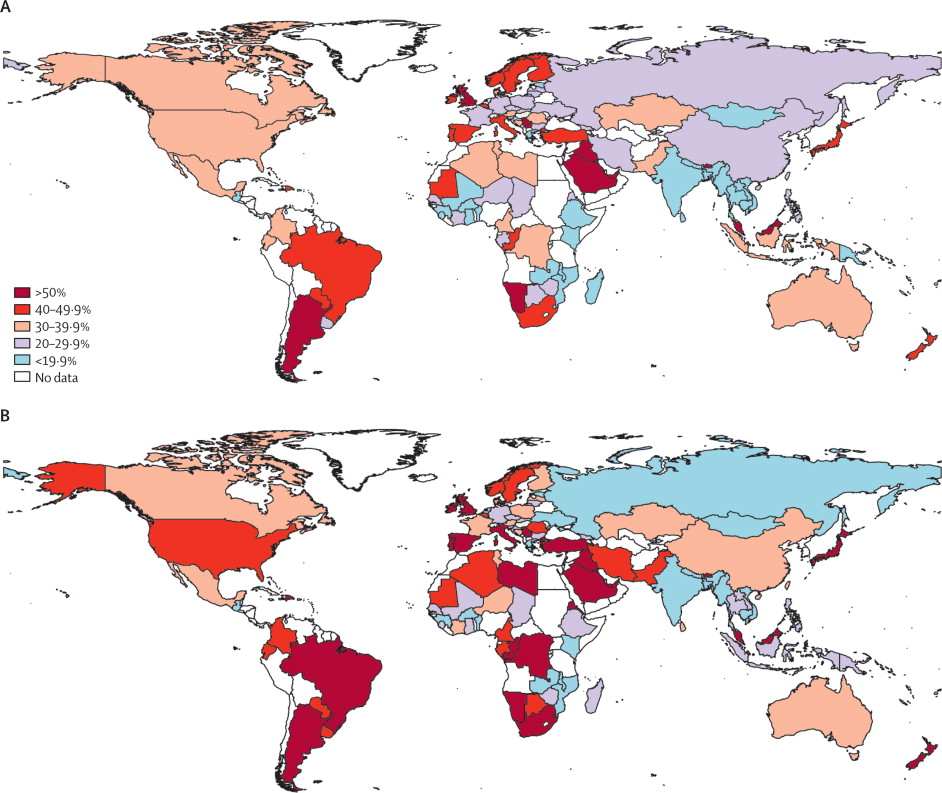
\includegraphics[width=1\textwidth]{Inactiviteit}
    \label{fig:inactivity}
\end{figure}

\textcite{Hallal2012} beschouwen 31,1\% van de wereldwijde bevolking als inactief. Dit wil zeggen dat, op het moment van onderzoek, bijna een derde van de volwassen wereldbevolking de vooropgestelde aanbevelingen van WHO, beschreven door \textcite{Bull2020}, niet haalt. Voor Europa ligt deze waarde zelfs op 34,8\% en zoals op Figuur \ref{fig:inactivity} te zien is, ligt België nog een stuk boven de gemiddelde Europese waarde met 40\% à 49,9\%.

\subsection{Invloed van beweging op mentale gezondheid}
Vele studies hebben aangetoond dat er endogene opioïden aangemaakt worden bij het sporten \autocite{Harber1984}. Endogene opioïden (endorfines, enkefalines en dynorfines) zijn peptiden die biochemische eigenschappen hebben die lijken op opiaten zoals heroïne en morfine. Vooral endorfine als gevolg van training wordt in verband gebracht met zowel fysiologische als psychologische veranderingen \autocite{Dishman2009}.

Deze chemische stoffen komen soms vrij als reactie van het menselijk lichaam op pijn, wat ervoor zorgt dat de pijnperceptie kan veranderen \autocite{Chaudhry2023, Dishman2009}. Daarnaast werden ze ook al geassocieerd met een toestand van plezier \autocite{Chaudhry2023}.

Daarnaast stellen \textcite{Mahindru2023} dat voldoende lichaamsbeweging kan helpen met het verbeteren van slaap, wat op zijn beurt zorgt voor het reguleren van normale hormonale en metabolische processen \autocite{Dolezal2017}. Te weinig slapen heeft zelfs een negatieve impact op de economie: het kost Amerikaanse bedrijven en gezondheidszorginstanties jaarlijks miljarden dollars \autocite{Dolezal2017}.


\subsection{Invloed van beweging op productiviteit}
Wanneer de algemene gezondheid van werknemers slecht is, brengt dit kosten mee voor het bedrijf. \textcite{Sjoegaard2016} beschrijven hoe deze kosten gerelateerd zijn aan de mentale en fysieke afwezigheid van werknemers tijdens het werk, met een verminderde productiviteit tot gevolg. Echter, voor personen die sedentair werk uitvoeren en voornamelijk aan een computer werken, zorgt een verhoogde hoeveelheid sport tijdens de vrije tijd voor minder stress en meer energie op de werkvloer \autocite{Hansen2009}. Daarnaast wordt er voor mensen die in de gezondheidszorg werken, na drie maanden consistent sporten, 8\% productiviteitsstijging waargenomen \autocite{Sjoegaard2016}.

Op die manier leidt het invoeren van regelmatige beweging, door middel van op voorhand opgestelde oefeningen en een zorgvuldige begeleiding, volgens \textcite{Cancelliere2011} tot een positief effect op de productiviteit. In die mate dat \textcite{Sjoegaard2016} stellen dat dit effect de eventuele uitgaven in verband met sportactiviteiten overstijgt.

\section{Gamification}
Volgens \textcite{Deterding2011} is gamification te beschrijven als het gebruiken van speldesignelementen in een niet-spelgerelateerde context.

De laatste jaren wint gamification aan populariteit als manier om gebruikersengagement te ondersteunen en als positieve manieren in het gebruik van diensten te verbeteren \autocite{Hamari2014}.

Gamification bestaat uit drie hoofdonderdelen: de gebruikte techniek, de psychologische uitkomsten en de verdere invloed op het gedrag \autocite{Hamari2014}. Daarnaast zijn sociale aspecten ook essentieel: door het ontstaan van een competitie streven mensen ernaar erkenning te ontvangen \autocite{Hamari2013}.

\subsection{Meest gebruikte technieken}
Volgens \textcite{Legaki2020} kunnen gamificationtechnieken in drie types gecategoriseerd worden: focus op prestaties of uitdagingen, onderdompeling in een verhaal en gebaseerd op sociale interactie.

\subsubsection{Punten en scoreborden}
Volgens \textcite{Hamari2014} zijn punten en scoreborden de meest voorkomende technieken. Punten worden toegekend voor het uitvoeren van vooropgestelde taken, ze focussen dus op prestatie. Aan de hand van deze punten kunnen scoreborden worden opgesteld. Deze scoreborden kunnen de resultaten van meerdere gebruikers tegen elkaar opzetten, wat voor een onderlinge competitie zorgt. Ditzelfde principe kan ook toegepast worden op eigen resultaten, waarbij een gebruiker steeds zichzelf probeert te overtreffen.

\subsubsection{Uitdagingen en badges}
Badges en uitdagingen binnen een spelcontext, tonen veel gelijkenissen met bepaalde marketing tools, zoals klantenkaarten waarop stempels verzameld moeten worden \autocite{Nunes2006}. Dit fenomeen noemen \textcite{Nunes2006} het ``begiftigde vooruitgangseffect'', hierbij zullen mensen meer volharding tonen om een doel te bereiken als ze op een kunstmatige manier vooruitgang kunnen merken richting dat doel.

Een voorbeeld van dit type gamification is \href{https://foursquare.com/}{Foursquare}, deze dienst is gebaseerd op mensen die badges ontgrendelen door bepaalde locaties te bezoeken in de ``echte'' wereld \autocite{Hamari2011}. Maar ook Apple Conditie past dit principe toe met hun badges \autocite{Ha2020}. Op figuur \ref{fig:apple_badges} is zichtbaar hoe deze medailles onderverdeeld worden in meerdere categorieën.

\begin{figure}[h]
    \caption[Badges in de Apple Conditie applicatie]{Een voorbeeld van badges in de Apple Conditie applicatie (Macworld, \href{https://www.macworld.com/article/231140/how-to-get-all-of-the-apple-watch-activity-challenge-badges.html}{2019})}
    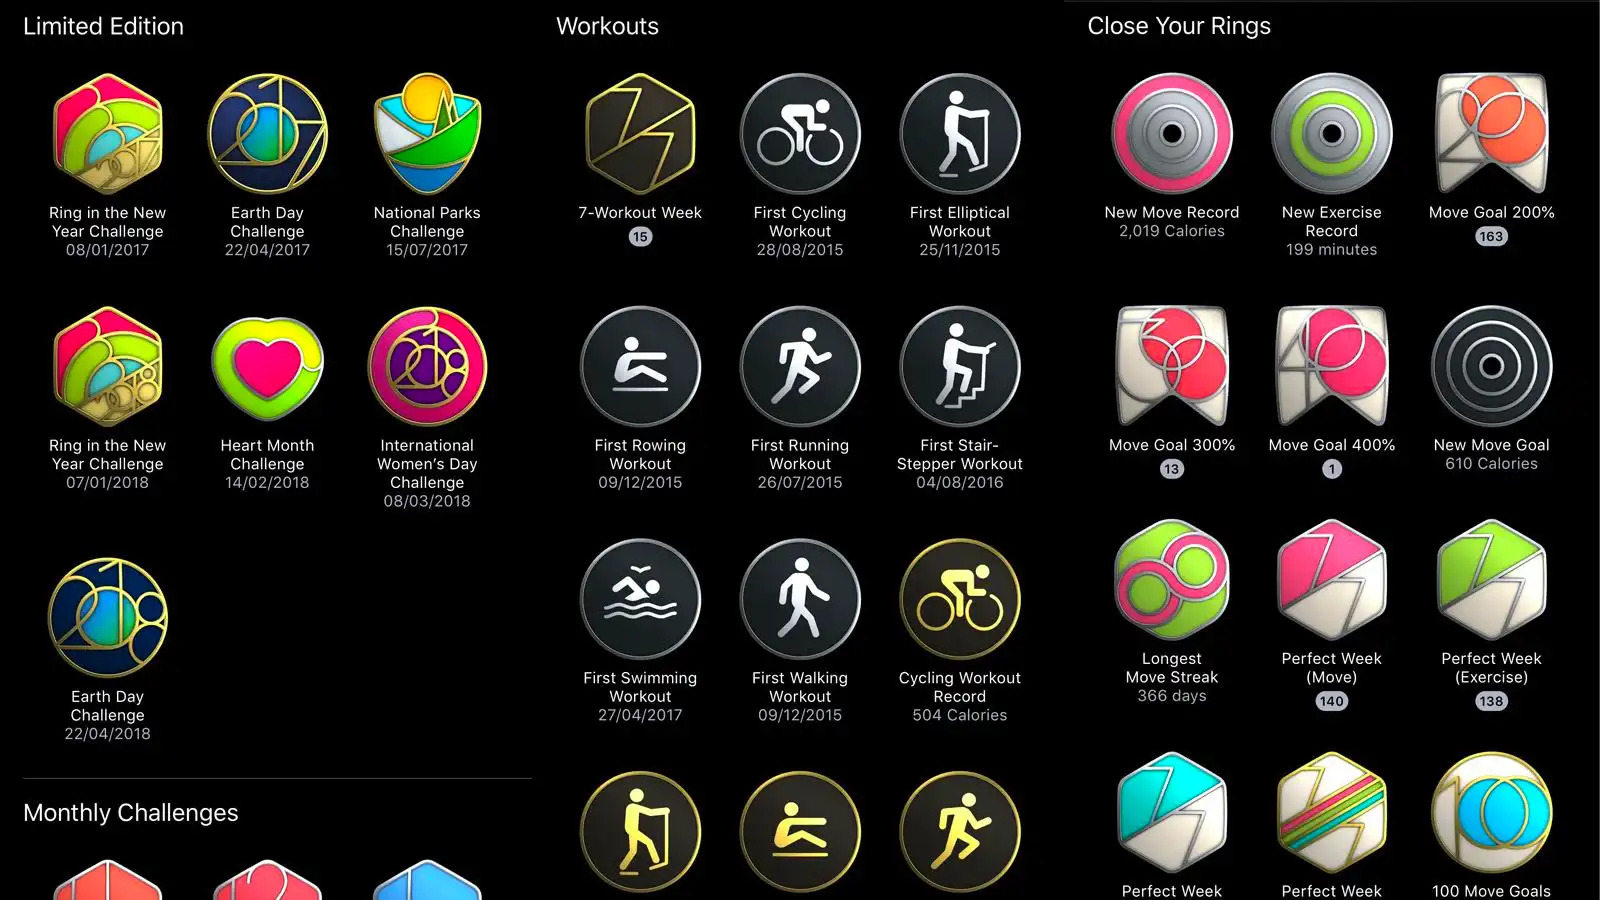
\includegraphics[width=1\textwidth]{AppleBadges}
    \label{fig:apple_badges}
\end{figure}

\subsubsection{Levels}
Levels worden gebruikt om gebruikers continu te blijven uitdagen en betrokken te houden \autocite{Dong2012}. Deze techniek is vooral gericht op persoonlijke motivatie en het stimuleren van de eigen vooruitgang en net om die reden is het uitermate geschikt voor het onderwijs \autocite{ManzanoLeon2021}.
\textcite{ManzanoLeon2021} beschrijven hoe deze techniek voldoet aan de ``Self-Determination Theory'' (SDT), een concept waarin drie psychologische behoeften oorzaak zijn voor intrinsieke motivatie: autonomie, competentie en verbondenheid met anderen. Gebruikers kunnen namelijk op een autonome manier evolueren doorheen deze levels, ze voelen zich competent wanneer ze slagen en gezien iedereen dezelfde niveaus doorloopt, ontstaat er een gevoel van verbondenheid.

\subsubsection{Storytelling}
Verhalen kunnen gebruikt worden om onderdompeling en engagement te creëren \autocite{ManzanoLeon2021}. Daarnaast kan de samenhang van een team er ook mee verbeterd worden: ieder krijgt dan een rol die zijn eigen bijdrage aan het verhaal moet leveren \autocite{ManzanoLeon2021}.

\textcite{Marczewski2015} stelt dat het bij storytelling ook zeer belangrijk is om zowel geloofwaardig te zijn, binnen de regels te blijven van het universum dat gecreëerd wordt, als er voor te zorgen dat elke keuze die gemaakt moet worden, wel degelijk een bijdrage levert aan het geheel. Wanneer een gebruiker namelijk op het einde het gevoel heeft dat diens keuzes nutteloos waren voor het eindresultaat, zal dit vaak resulteren in een teleurstelling in het product \autocite{Marczewski2015}.

Om dit te vermijden, stelt \textcite{Duster1990} dat het beter is om niet noodzakelijke elementen te verwijderen uit een verhaal: ``een geweer dat tijdens het eerste bedrijf van toneelstuk, moet gebruikt worden tegen het derde [bedrijf]''.

Storytelling is voor deze casus minder van toepassing, het wordt eerder gebruikt in het onderwijs \autocite{Schmoelz2018}.

\subsubsection{Beloningen}
Beloningen kunnen al dan niet in combinatie met één van de hierboven vermeldde technieken gebruikt worden. Ze kunnen bijvoorbeeld bestaan uit, maar daarom niet gelimiteerd worden tot, een donatie aan een gekozen goed doel of een eervolle vermelding op een intern bedrijfsevenement.
Volgens \textcite{Lewis2016} zijn tastbare beloningen echter niet altijd de beste optie, ze kunnen er namelijk voor zorgen dat de ontwikkeling van intrinsieke motivatie afgeremd wordt, terwijl deze net zorgt voor behoud van gedrag op lange termijn. Punten en badges kunnen echter ook als beloning beschouwd worden, en zouden dit effect niet hebben \autocite{Lewis2016}.

\subsection{Psychologische aspecten}
Gamification is sterk gebaseerd op psychologie. Wanneer psychologische aspecten bevraagd zijn, is er vooral gefocust op motivatie, attitude en plezier \autocite{Hamari2014}. \textcite{Cheong2013} werkte een online quiz uit die gamification gebruikt, met als doel om studeren aan te moedigen door het leuker te maken. Uit een bevraging  na de quiz bleek dat 40,79\% van de deelnemers enthousiast en 46,05\% van de deelnemers tevreden was tijdens de quiz. Daarenboven was het merendeel (77,63\%) van de deelnemers voldoende gemotiveerd om de quiz te vervolledigen.

\subsubsection{Hiërarchie van behoeften}
Een van de oudste en meest bekende motivatietheorieën is afkomstig van psycholoog Abraham Maslow \autocite{Richter2014}. Volgens hem handelen mensen met als doel om fysieke en psychologische behoeften te bevredigen. Maslow spreekt over vijf niveaus van noden die menselijke activiteiten aansturen, gaande van fysieke tot persoonlijke behoeften (zie figuur \ref{fig:people-hierarchy}) \autocite{Lilienfeld2014}.

Op basis van dit model, hebben \textcite{Siang2003} een hiërarchie gemaakt die op gamers van toepassing is (zie figuur \ref{fig:gamers-hierarchy}).
Hiervoor geldt dat de onderste levels moeten worden vervuld voor de hogere niveaus in de piramide \autocite{Richter2014}.
Eerst zoeken spelers naar informatie om de regels van het spel te begrijpen. Daarna heeft een speler nood aan veiligheid om door te zetten en mogelijks te winnen. Ten derde moet een speler zich erbij horen voelen, waarna die zich goed moet voelen tijdens het spelen van het spel, er moet een gevoel van waardering aanwezig zijn. Op het volgende level willen spelers grotere uitdagingen en willen ze meer begrijpen over het spel en diens strategieën. Het voorlaatste niveau gaat over de wens voor bijvoorbeeld goede graphics, bijpassende muziek en geluidseffecten. Ten slotte willen spelers een soort van perfectie bereiken binnen deze virtuele wereld, waarin alles kan en mag binnen de regels van het spel \autocite{Greitzer2007, Siang2003}.

Bij het implementeren van gamification in een sportplatform is het dus belangrijk om ervoor te zorgen dat aan de onderste zes niveaus (zie figuur \ref{fig:gamers-hierarchy}) voldaan is, zodat mensen zichzelf ook willen verbeteren via het platform.

\begin{figure}[h]
    \caption[Behoeften-hiërarchie algemeen]{De  niveaus van behoeften die menselijke activiteiten aansturen \autocite{Lilienfeld2014}}
    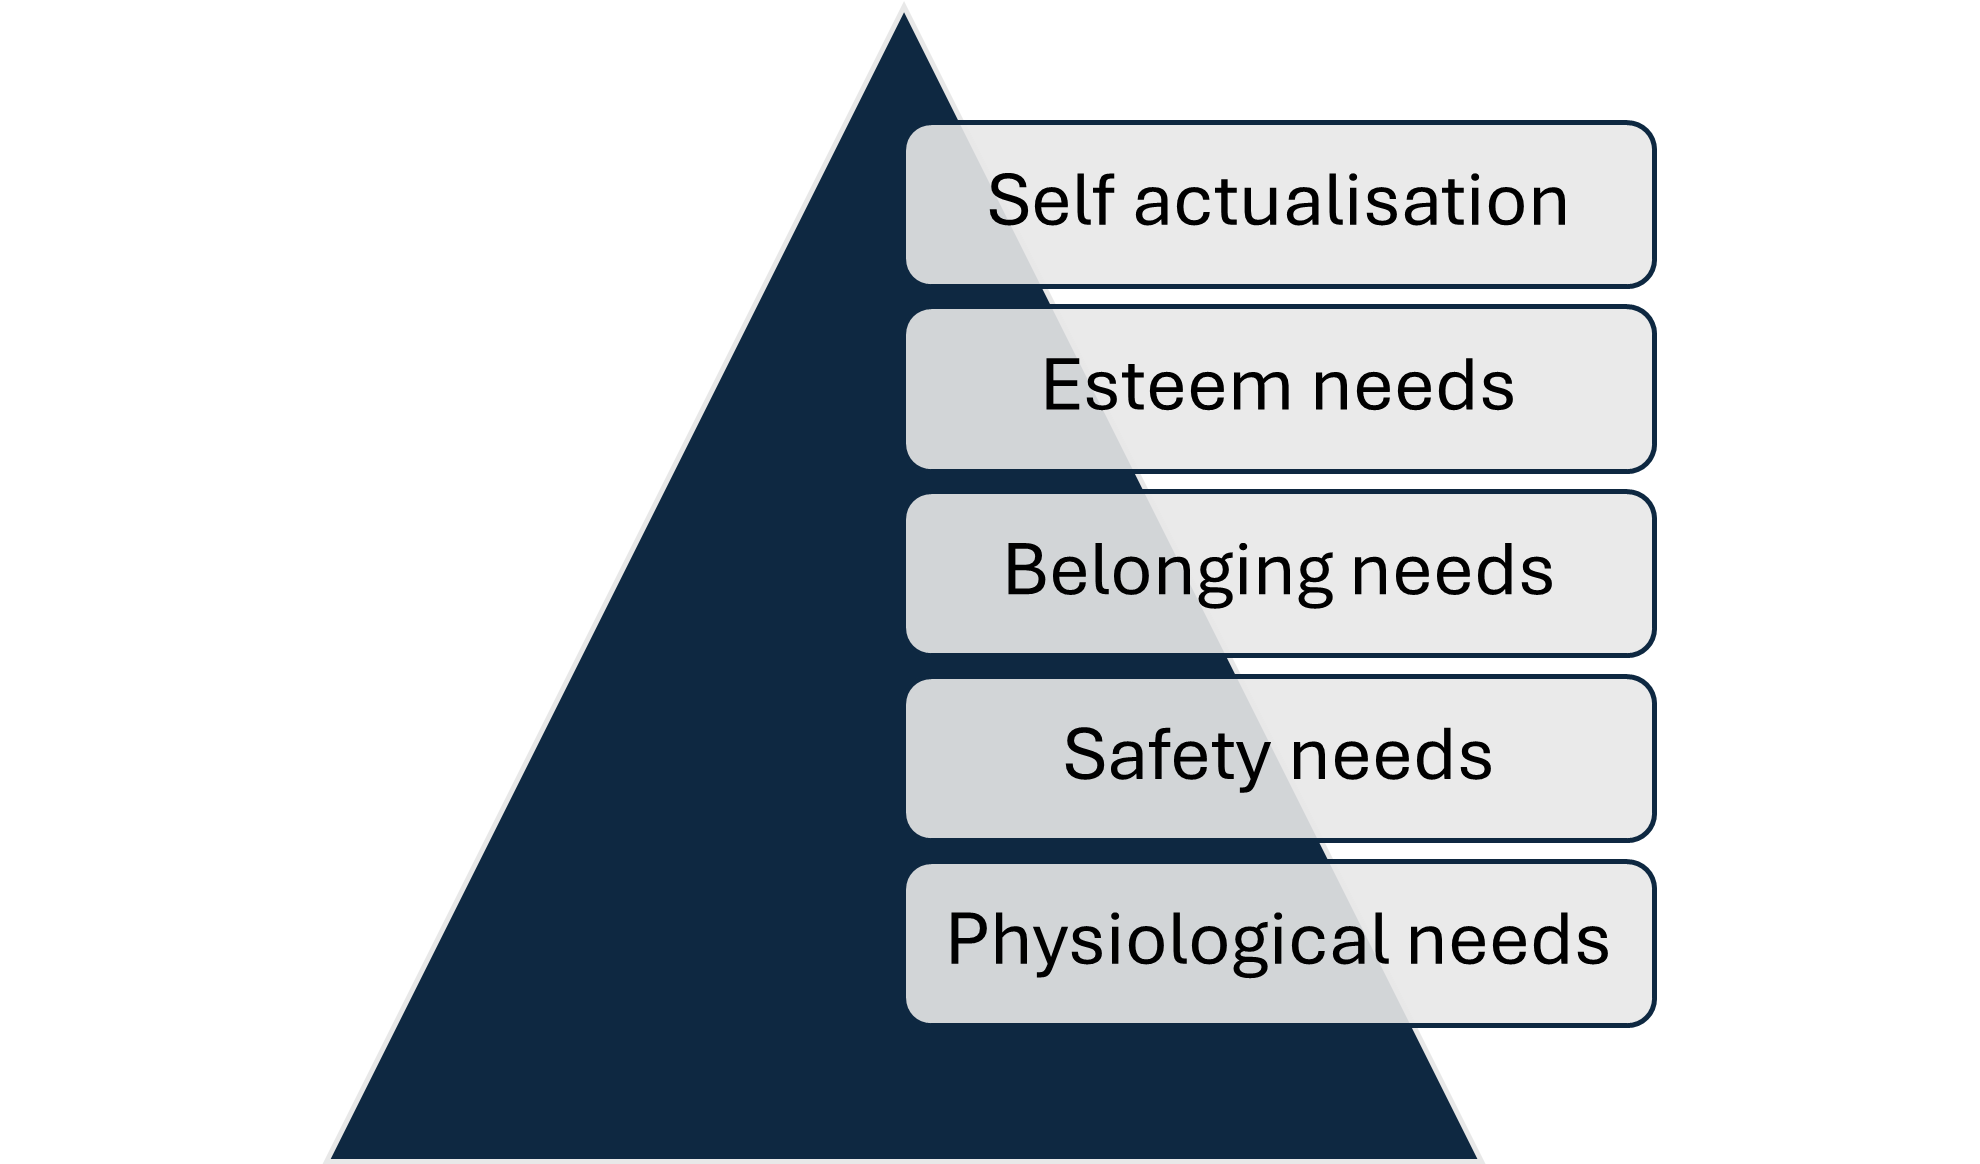
\includegraphics[width=1\textwidth]{PyramidPeople}
    \label{fig:people-hierarchy}
\end{figure}


\begin{figure}[h]
    \caption[Behoeften-hiërarchie gamers]{De hiërarchie van behoeften van gamers \autocite{Richter2014}}
    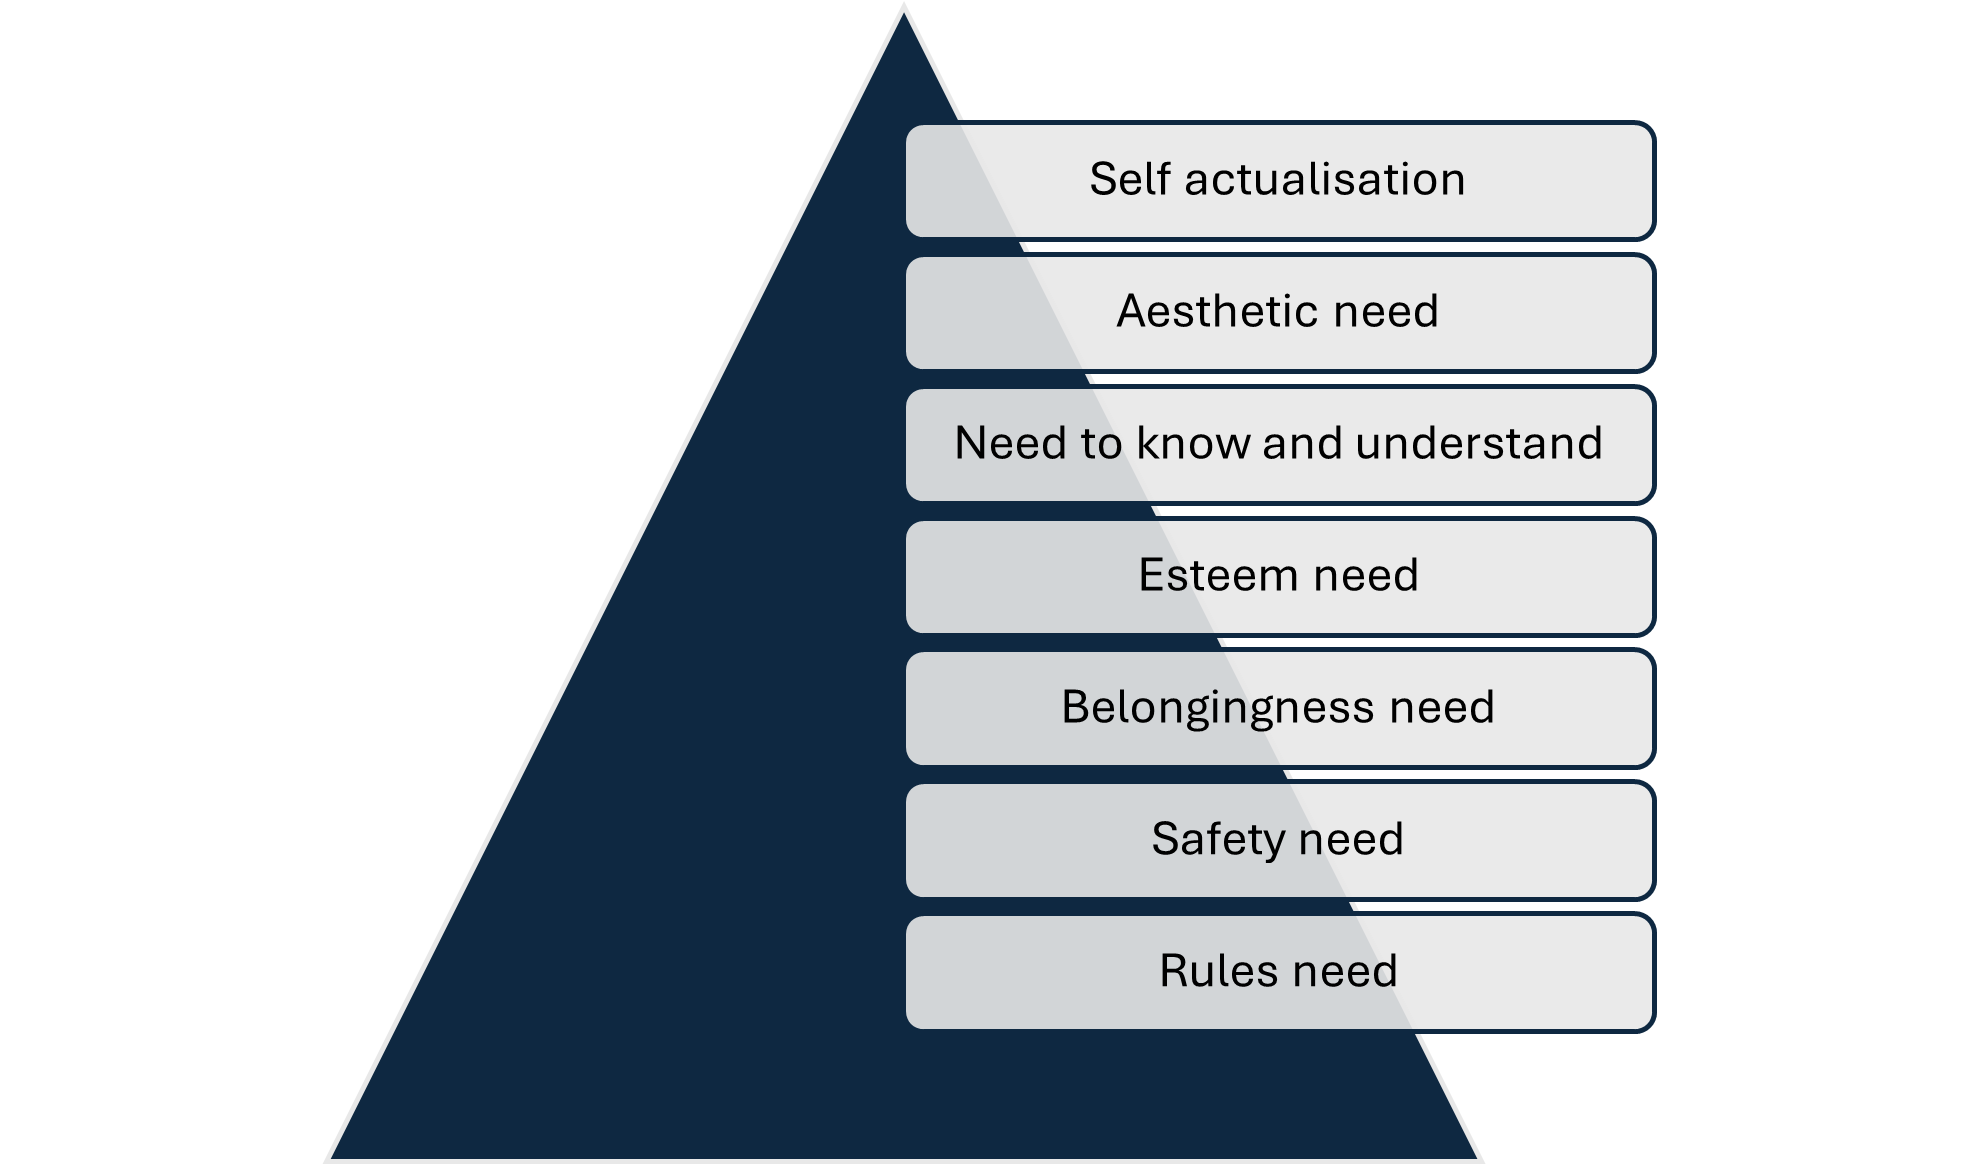
\includegraphics[width=1\textwidth]{PyramidGamers}
    \label{fig:gamers-hierarchy}
\end{figure}

\subsection{Invloed op gedrag}
\textcite{Kari2016} stellen dat gamification in sportapplicaties een positieve invloed heeft op de intrinsieke bewegingsmotivatie, wat ervoor zorgt dat gebruikers gaan handelen naar een bepaald doelgedrag. \textcite{PoloPena2020} bevestigen dit, maar voegen hier wel aan toe dat gamification een grotere invloed heeft op vrouwen dan op mannen, en op oudere mensen dan op jongere gebruikers.

Studies van \textcite{Hamari2013a} hebben aangetoond dat de resultaten van gamification mogelijks niet voor alle gebruikers op lange termijn doeltreffend zijn, en de invoering ervan mogelijks niet op iedereen het gewenste effect heeft.
Anderzijds zal het verwijderen van spelelementen uit een dienst schadelijke gevolgen hebben voor de gebruikers die wel nog betrokken zijn tot het gamification-aspect: zo kan een gebruiker plots al zijn vooruitgang of verdiende badges verliezen.

\subsubsection{Geslacht}

\textcite{Venkatesh2000} bespreken hoe het proces om een beslissing te maken, verschilt per geslacht. Zo is bijvoorbeeld gevonden dat mannen meer instrumenteel of proactief gedrag vertonen, wat wilt zeggen dat ze vaker in de aanval of verdediging gaan om zo anderen onder druk te zetten om uiteindelijk op die manier hun doel te bereiken of zin te krijgen \autocite{Spence1980}. Daarnaast stellen \textcite{Hoffman1972, Minton1980} dat ze ook meer taak- en prestatiegericht zijn dan vrouwen. Daartegenover staat dat voor vrouwen de behoefte voor verbondenheid een belangrijkere rol speelt \autocite{Hoffman1972} en ze volgens \textcite{Minton1980, Spence1980} ook meer gericht zijn op sociale relaties. Dit betekent dat vrouwen vatbaarder zijn voor sociale invloed van bijvoorbeeld gamification.

In de huidige online wereld met al diens sociale features, blijkt dat vrouwen de meer sociaal gemotiveerde gebruikers zijn, terwijl mannen eerder focussen op pragmatisch gebruik \autocite{Haferkamp2012, Muscanell2012}. Daartegenover staat dat in sommige studies van \textcite{Wang2008} geconcludeerd wordt dat mannen, in bepaalde contexten zoals online leren, beïnvloed worden door sociale factoren. \textcite{Koivisto2014} besluiten hierover dat het invoeren van sociale features essentieel is als men ook vrouwelijke gebruikers wil betrekken.

\subsubsection{Leeftijd}

Wanneer ouderen beslissen over hun intentie om een technologie al dan niet te gebruiken, hechten ze minder belang aan het nut van de technologie dan jongeren \autocite{Venkatesh2003}. Net als vrouwen, worden ouderen ook meer beïnvloed door sociale invloeden dan jongere gebruikers. Dit is mogelijk te wijten aan een hogere associatienood \autocite{Morris2000, Venkatesh2003, Wang2008}.

Over het algemeen ervaren oudere generaties meer computerstress en schatten ze daardoor hun IT-vaardigheden slechter in \autocite{Chung2010}. Ze hechten ook meer belang aan het gemak in gebruik van een systeem: de afweging tussen het waargenomen gebruiksgemak en het nut en de mogelijke voordelen wordt belangrijker naarmate een gebruiker ouder wordt, concluderen \textcite{Melenhorst2001}.

\textcite{Arning2007, Czaja2006} stellen wel dat gamification, als die sociale verbondenheid en zelfredzaamheid bevordert, het ook mogelijk maakt om gebruikers van gevorderde leeftijd te betrekken bij diensten.

\subsection{Sociale aspecten}
Er zijn twee belangrijke sociale aspecten om in acht te nemen wanneer gamification geïmplementeerd wordt.

Enerzijds is er erkenning, wat beschreven kan worden als de sociale feedback die gebruikers krijgen op hun gedrag \autocite{Cheung2011}.
Wanneer een dienst, zoals het aanbieden van een platform met gamification, erkenning van de andere gebruikers oplevert, wordt die dienst positiever ervaren \autocite{Preece2001}.
\textcite{Hamari2013} suggereren dat er vervolgens, als gevolg van de ontvangen erkenning, een bepaalde bereidheid ontstaat om de erkenning wederkerig te maken. Hierdoor zal de tegenpartij ook op zijn beurt de dienst positiever ervaren.

Anderzijds is er sociale invloed, wat verwijst naar de perceptie van een individu over het belang dat anderen hechten aan een bepaald doelgedrag en of ze verwachten dat iemand dat gedrag zal vertonen \autocite{Ajzen1991}. Specifiek voor een platform dat gamification implementeert, kan er sociale invloed ontstaan door het zien van wat andere gebruikers op het platform presteren. Hierdoor wordt namelijk een verwachtingspatroon gecreëerd en zetten gebruikers elkaar aan tot het behalen van een bepaald doelgedrag, zoals vaker sporten.

Een keerzijde van deze sociale interactie, kan zijn dat het mensen afschrikt. Het kan namelijk zo zijn dat mensen die pas beginnen met sporten zichzelf zullen spiegelen aan anderen die al regelmatig sportten. Hier zal dus de nodige aandacht aan moeten worden besteed.

\section{Bestaande sportapplicaties}
Hieronder volgt een diverse greep uit de bestaande mobiele en desktop sportapplicaties en -platformen en welke spelelementen daarin gebruikt worden.

\href{https://www.strava.com/}{Strava} is een applicatie waarmee gebruikers hun sportprestaties kunnen bijhouden. \textcite{Barratt2017} stelt dat deze applicatie gamification toepast in de vorm van uitdagingen en persoonlijke trainingsvooruitgang.

Een tweede voorbeeld is de loopapplicatie \href{https://www.nike.com/be/en/nrc-app}{Nike Run Club}, met meer dan 10 miljoen downloads\footnote{\href{https://bootcamp.uxdesign.cc/how-the-nike-run-club-app-got-runners-hooked-2850c7654fc5}{How the Run Club App got runners hooked - Leevey}} op de Google Play Store en de App Store. Deze applicatie maakt het mogelijk voor lopers om een looptraining vast te leggen, punten te verdienen en andere gebruikers uit te dagen. Daarnaast kunnen ze eigen doelstellingen aanmaken en delen, zodat samen naar een gezamenlijk doel gewerkt kan worden \autocite{StaalnackeLarsson2013}.

Daarnaast bestaat ook \href{https://connect.garmin.com/}{Garmin Connect}. Het verschil met de vorige twee applicaties, is dat dit platform enkel voor gebruikers met een Garmin-toestel bedoeld is. Deze applicatie focust vooral op badges \autocite{Ilhan2019}. Het behalen van zulke badge kan dan punten opleveren en de mogelijkheid geven tot het behalen van nieuwe, meer uitdagende badges. Om negatieve gevoelens van frustratie op een mindere dag tegen te gaan, krijgt de gebruiker de optie om andere, niet fysieke activiteiten, uit te voeren om ook dan punten te verdienen.

Een laatste voorbeeld is \href{https://support.apple.com/nl-be/guide/iphone/ipha5dddb411/ios}{Apple Conditie}. Dit platform kan enkel gebruikt worden door gebruikers met een Apple toestel. Zoals eerder aangehaald, focust deze applicatie op het behalen van medailles, het bijhouden van persoonlijke vooruitgang en indien gewenst ook sociale gamification door het delen van sportieve prestaties binnen de applicatie.

Voor deze casus is echter een platform nodig dat een competitie opzet die gericht is op mensen in een zittend beroep. Door de focus op deze doelgroep, zal de gamification hierop afgestemd zijn en zullen mensen minder snel gedemotiveerd zijn. Dergelijke applicatie zal ontwikkeld worden in een volgende fase van het onderzoek.

%%=============================================================================
%% Methodologie
%%=============================================================================

\chapter{\IfLanguageName{dutch}{Methodologie}{Methodology}}%
\label{ch:methodologie}

Dit hoofdstuk schetst in grote lijnen hoe het onderzoek verlopen is en kadert hoe alle elementen van deze bachelorproef samenhangen.

\section{Voorbereidend onderzoek}
Uit de literatuurstudie is reeds gebleken dat er, ondanks het bewezen belang van voldoende beweging, te veel fysieke inactiviteit is bij volwassenen. Voorgaande onderzoeken, zoals onder andere de paper van \textcite{Kari2016}, stellen vast dat de intrinsieke bewegingsmotivatie kan worden gestimuleerd door een sportplatform dat gebruik maakt van gamification. Gezien \textcite{Hamari2013} echter stellen dat dit gewenste effect niet op iedereen van toepassing is, wenst deze bachelorproef te onderzoeken of de eerdere bevindingen kunnen worden bevestigd bij personen met een sedentaire job.

Om dit uit te voeren, zal eerst een diverse groep werknemers, die een sedentaire job uitoefenen, worden geselecteerd. Daarna zullen zij worden onderworpen aan een eerste bevraging.

Enerzijds is het de bedoeling te achterhalen in welke mate sport en beweging een rol speelt in hun dagelijkse leven op het moment van het interview. Anderzijds heeft deze ook als doel te achterhalen in welke mate en op welke manieren deze werknemers gestimuleerd kunnen worden om meer te gaan sporten. Dit laat toe om de gamificationtechnieken te identificeren die van toepassing kunnen zijn op deze specifieke casus.

Op basis van al de ontvangen informatie kan bepaalde theorie uit de literatuurstudie reeds worden afgetoetst. Echter vergt de onderzoeksvraag van deze bachelorproef verdergaand onderzoek, zodat op basis van de verkregen inlichtingen de vereisten van de sportapplicatie zijn opgesteld, en de ontwikkeling ervan is begonnen.

\section{Ontwikkeling en ingebruikname van ``Move-it!''}

Steunend op de bekomen resultaten uit zowel de literatuurstudie als de analyse van de gebruikersinterviews, werd een sportapplicatie genaamd ``Move-it!'' ontwikkeld. Het technisch aspect van de ontwikkeling en de geïncorporeerde competitie bevorderende gamificationtechnieken worden verder besproken in hoofdstuk \ref{ch:proofofconcept}.

Deze ``Proof Of Concept'' (POC) dient om een antwoord te bieden op de onderzoeksvragen: heeft het competitief sportplatform, dat gebruik maakt van gamification, een positieve invloed op het sportgedrag van werknemers in een sedentaire job? Welke gamificationtechnieken hebben het meeste succes? Zijn er technieken die een negatief effect hebben?

Om deze vragen te beantwoorden, hebben na een gebruiksperiode van vier weken van "Move-it!" gebruikersinterviews plaatsgevonden, met dezelfde personen die voor aanvang van de ontwikkelings- en gebruiksfase geïnterviewd zijn.
Daarbij zijn de vragen quasi identiek gebleven, maar putten de deelnemers voor het beantwoorden van de tweede vragenlijst uit hun ervaringen met het sportplatform. Die ervaringen gingen vooraf door een uitleg over de precieze werking van "Move-it!", waardoor aan de eerste behoefte, zoals beschreven door \textcite{Siang2003} (zie \ref{ssec:werking-gamification}), werd voldaan. De vastgelegde hiërarchie der behoeften in een spelcontext stelde namelijk dat er eerst nood is aan regels om het spel te begrijpen. Daarna werden wekelijkse herinneringen om de gepresteerde uren in te geven, bezorgd. Deze sportgegevens moeten in combinatie met de antwoorden van de vragenlijsten een grondige analyse en daaropvolgende conclusie toelaten, wat in de volgende sectie zal besproken worden.

\section{Analyse van de cijfers}

Zowel de bekomen sportgegevens als de data uit de bevragingen zijn gebruikt om een analyse uit te voeren.

Bij de analyse van de bevragingen wordt er vooral gepeild naar:
\begin{itemize}
    \item de mate van beweging van deelnemers,
    \item wat in de weg staat om meer te bewegen,
    \item welk gevoel gamification teweegbrengt,
    \item wat belangrijk is in een sportapplicatie.
\end{itemize}

In de sportgegevens wordt er vooral gezocht of er een evolutie merkbaar is binnen de tijdspanne van vier weken.

Deze analyse leidt uiteindelijk tot de conclusie van dit onderzoek, die vergeleken wordt met de hypothese die werd opgesteld op basis van eerder onderzoek.

Tenslotte volgt uit deze analyse ook een overzicht van welke mogelijkheden tot toekomstig onderzoek er zijn.

%% TODO: In dit hoofstuk geef je een korte toelichting over hoe je te werk bent
%% gegaan. Verdeel je onderzoek in grote fasen, en licht in elke fase toe wat
%% de doelstelling was, welke deliverables daar uit gekomen zijn, en welke
%% onderzoeksmethoden je daarbij toegepast hebt. Verantwoord waarom je
%% op deze manier te werk gegaan bent.
%%
%% Voorbeelden van zulke fasen zijn: literatuurstudie, opstellen van een
%% requirements-analyse, opstellen long-list (bij vergelijkende studie),
%% selectie van geschikte tools (bij vergelijkende studie, "short-list"),
%% opzetten testopstelling/PoC, uitvoeren testen en verzamelen
%% van resultaten, analyse van resultaten, ...
%%
%% !!!!! LET OP !!!!!
%%
%% Het is uitdrukkelijk NIET de bedoeling dat je het grootste deel van de corpus
%% van je bachelorproef in dit hoofstuk verwerkt! Dit hoofdstuk is eerder een
%% kort overzicht van je plan van aanpak.
%%
%% Maak voor elke fase (behalve het literatuuronderzoek) een NIEUW HOOFDSTUK aan
%% en geef het een gepaste titel.





% Voeg hier je eigen hoofdstukken toe die de ``corpus'' van je bachelorproef
% vormen. De structuur en titels hangen af van je eigen onderzoek. Je kan bv.
% elke fase in je onderzoek in een apart hoofdstuk bespreken.

%\input{...}
%\input{...}
\chapter{\IfLanguageName{dutch}{Proof of concept}{Proof of concept}}%
\label{ch:proofofconcept}

\section{Gekozen technologieën}

\subsection{Framework}

Gezien de expertise van we are, is er voor het platform gekozen voor een responsive React\footnote{\href{https://react.dev/}{https://react.dev/}}-website. Hiervoor is gebruik gemaakt van TypeScript \footnote{\href{https://www.typescriptlang.org/}{https://www.typescriptlang.org/}}.

Voor de implementatie van authenticatie is er gebruik gemaakt van Auth0\footnote{\href{https://auth0.com/}{https://auth0.com/}}. De redenen waarom er voor Auth0 gekozen is, zijn: de mogelijkheid om aan te melden met een Google-account, makkelijke integratie in React en de mogelijkheid tot een gratis abonnement wanneer het aantal gebruikers onder de 7000 blijft, wat voor deze POC meer dan voldoende is.

\subsection{Component libraries}
Gezien de korte ontwikkeltijd die beschikbaar was, zijn Material UI Core\footnote{\href{https://mui.com/core/}{https://mui.com/core/}} en Material UI X\footnote{\href{https://mui.com/x/}{https://mui.com/x/}} component libraries gebruikt voor de ontwikkeling van deze website, om zo het ontwikkelproces te vergemakkelijken. Er is gekozen voor Material UI wegens diens universele look-and-feel, het ruime aanbod aan gratis componenten en de beschikbaarheid van verschillende grafiek-componenten. Daarnaast zijn deze componenten uitermate geschikt voor zowel mobiel als desktop gebruik.

\subsection{Databank}

Deze applicatie gebruikt een graafdatabank, meer specifiek Neo4J\footnote{\href{https://neo4j.com/}{https://neo4j.com/}}. Er is in deze situatie gekozen voor een graaf databank omdat het zeer simpel op te zetten is en er geen databank-schema ontworpen moet worden, wat het dus zeer simpel maakt om snel te ontwikkelen en gaandeweg eventueel zaken aan te passen indien nodig.

Daarnaast zal de analyse van de ingegeven sportdata ook makkelijker verlopen: er zullen geen complexe join-operaties aan te pas komen, wat bij een SQL-databank wel het geval zou zijn.

\subsection{Deployment}

De website wordt gedeployed met behulp van Vercel\footnote{\href{https://vercel.com/home}{https://vercel.com/home}}. De GitHub\footnote{\href{https://github.com/}{https://github.com/}}-repository van deze applicatie is gelinkt aan een Vercel-project, wat er voor zorgt dat de elke nieuwe commit op de main-branch steeds gedeployed zal worden. Dit maakt het zeer eenvoudig om te beheren. Move-it is te vinden op \href{https://move-it-ghent.vercel.app/}{https://move-it-ghent.vercel.app/}.

\section{Opbouw van de applicatie}

De applicatie is opgesteld op basis van de volgende bouwstenen: een centraal dashboard, een overzicht van eigen prestaties, een oplijsting van de teamleden en een profielpagina.

\subsection{Dashboard}
Op het dashboard is de meeste informatie te zien: zowel persoonlijke evolutie over één week en over drie weken als de team en persoonlijke ranking zijn er te vinden. Om kleinere teams evenveel kans te geven, houdt de teamranking rekening met de grote van het team bij de berekening.

\subsection{Persoonlijk overzicht}
Op het persoonlijk overzicht is een lijst van de gepresteerde activiteiten te zien (figuur \ref{fig:performances} en figuur \ref{fig:performancesMobile}), en kunnen gebruikers ook hun prestaties ingeven. Hier is voldoende ruimte voorzien voor de ingave van technische gegevens, zoals gemiddelde hartslag en hoogtemeters. Afhankelijk van het type activiteit, en wanneer een afstand en duur ingegeven zijn, berekent de applicatie ook een gemiddelde snelheid. Zo kunnen frequente sporters eventueel een vooruitgang opmerken.

\begin{figure}[h]
    \caption[Overzicht activiteiten website]{Overzicht van gepresteerde activiteiten in de applicatie, gezien vanop een laptop.}
    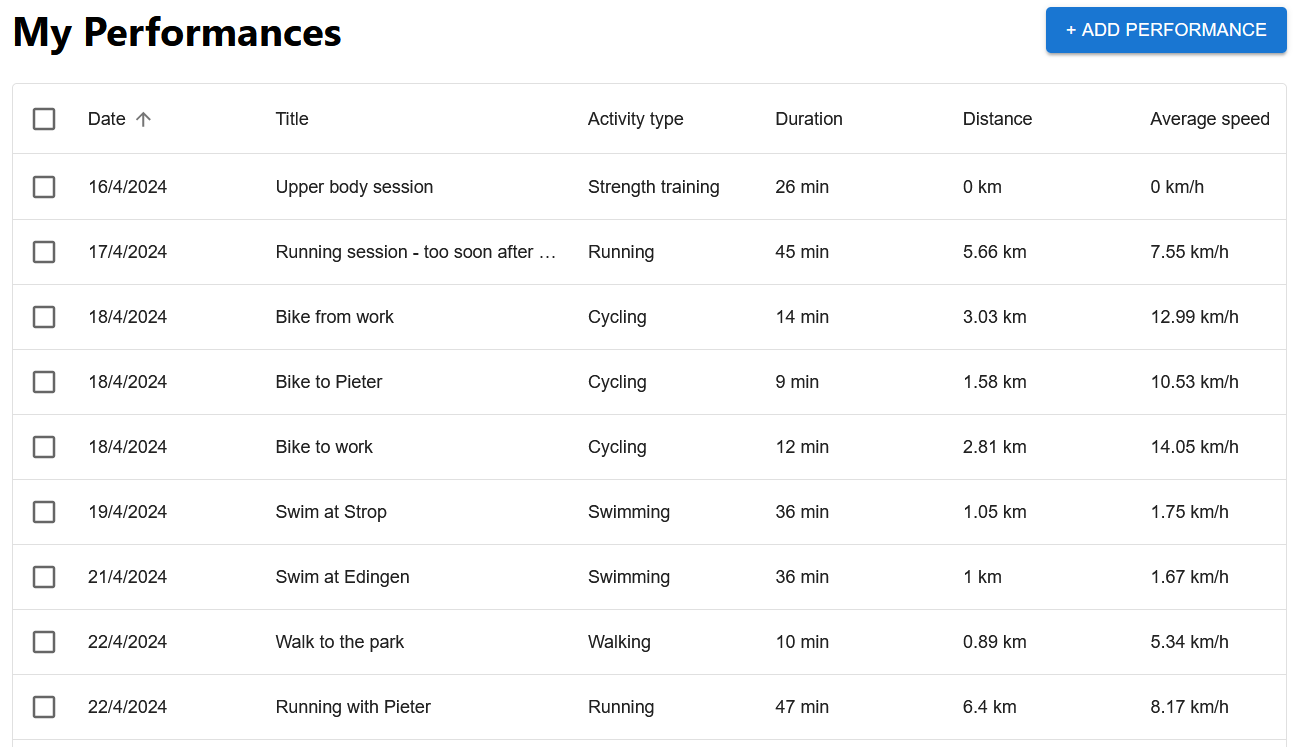
\includegraphics[width=1\textwidth]{MyPerformances}
    \label{fig:performances}
\end{figure}

\begin{figure}[h]
    \caption[Overzicht activiteiten website smartphone]{Overzicht van gepresteerde activiteiten in de applicatie, gezien vanop een smartphone.}
    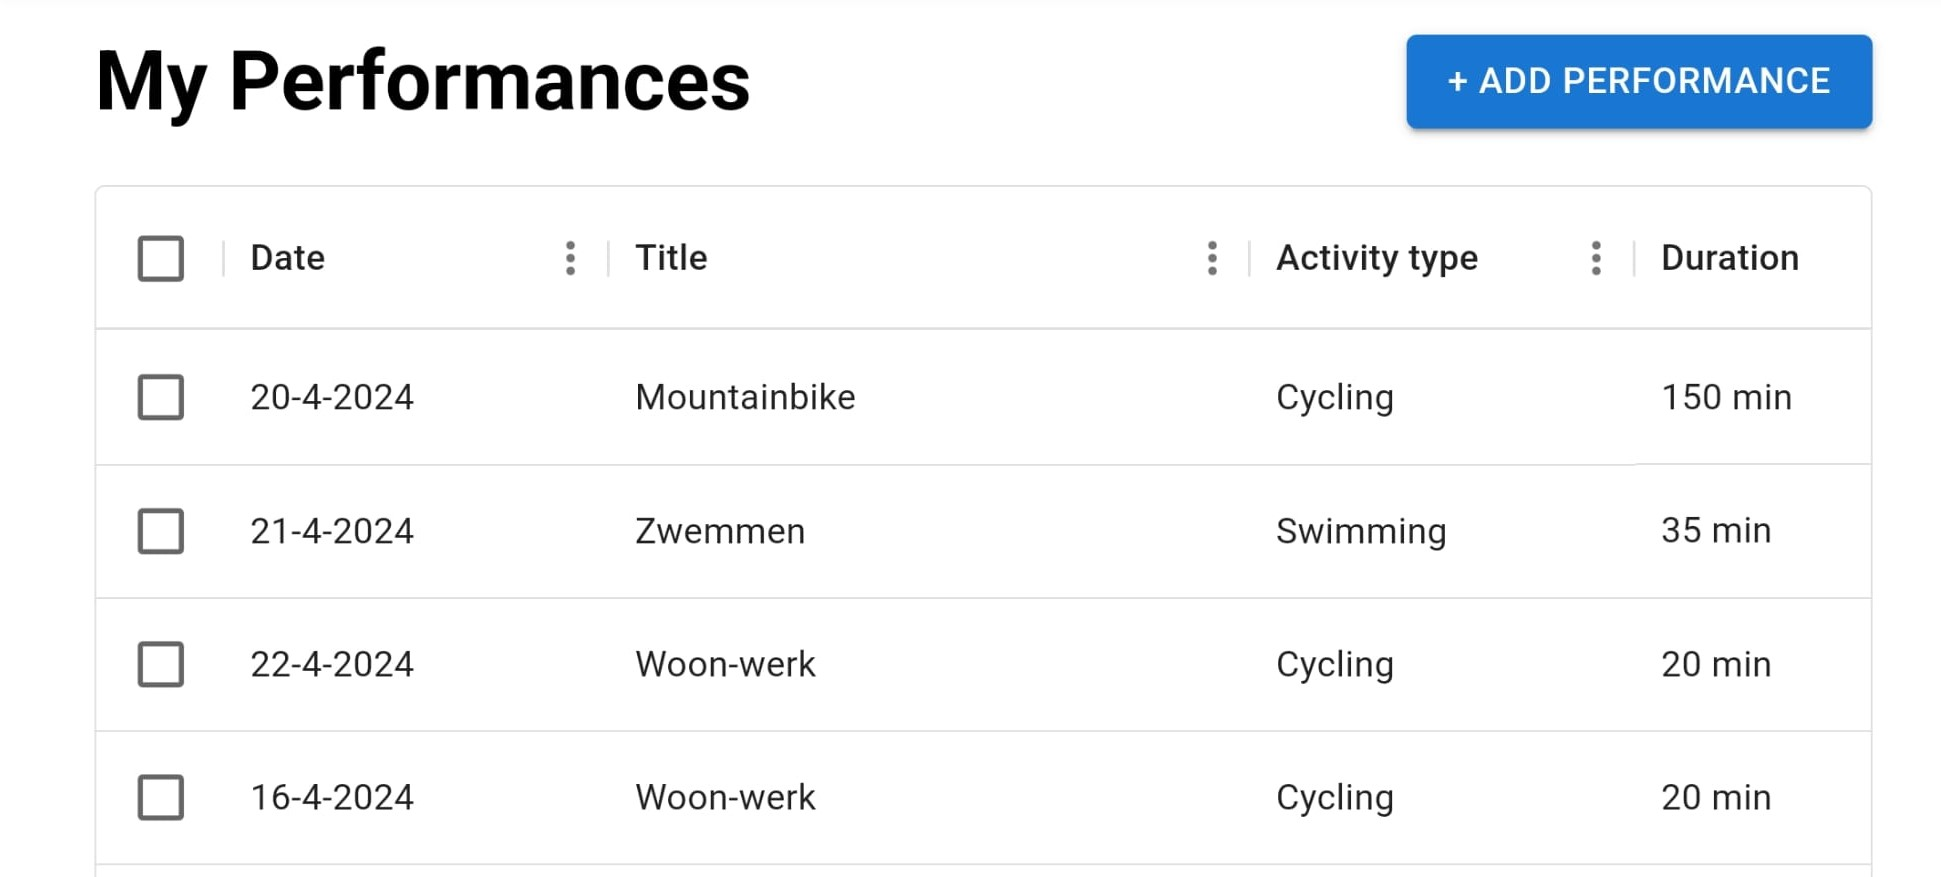
\includegraphics[width=1\textwidth]{MyPerformancesMobile}
    \label{fig:performancesMobile}
\end{figure}

\subsection{Teamoverzicht}

Dit overzicht is een simpele oplijsting van alle teamleden waartoe de aangemelde gebruiker behoort.

In de toekomst zou dit uitgebreid kunnen worden met een overzicht van de prestaties van een team, zodat er ook binnen een team gamification speelt en wat mogelijks tot meer motivatie kan leiden.

\subsection{Profiel pagina}

Op deze pagina kan een gebruiker een avatar, team en naam kiezen waarmee die weergegeven wordt.

\chapter{\IfLanguageName{dutch}{Analyse van de cijfers}{Analysis of the figures}}%
\label{ch:analyse}

Allereerst heeft er een online vragenlijst plaatsgevonden. Daarna is de POC in gebruik genomen door diezelfde mensen als zij die de vragenlijst ingevuld hebben. Tenslotte is nogmaals een vragenlijst uitgestuurd om eventuele veranderingen of evoluties op te merken.

De éénentwintig bevraagde mensen zijn allen werkzaam in een sedentaire job. 42.9\% van de respondenten zijn tussen de 18 en 25 jaar oud, 42.9\% tussen de 25 en 35 jaar oud en de overige 14.3\% zijn tussen de 35 en 45 jaar oud. Deze bachelorproef kan dus geen conclusies trekken over mensen die zich buiten deze leeftijdsgroepen bevinden.

\section{Resultaten voor gebruik van Move-it!}

\subsection{Beweging}
Slechts 33.3\% van de bevraagde personen is tevreden met diens hoeveelheid dagelijkse beweging (zie figuur \ref{fig:dagelijkseBeweging}).

\begin{figure}[h]
    \caption[In welke mate vindt u van uzelf dat u dagelijks voldoende beweegt (op een schaal van 1 tot en met 5, gaande van 1 voor absoluut te weinig bewegen, tot en met 5 voor meer dan voldoende bewegen)?]{In welke mate vindt u van uzelf dat u dagelijks voldoende beweegt (op een schaal van 1 tot en met 5)?}
    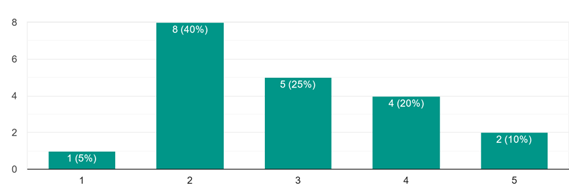
\includegraphics[width=1\textwidth]{DailyMovement}
    \label{fig:dagelijkseBeweging}
\end{figure}

Volgens de WHO moeten volwassenen tussen de 18 en 64 jaar oud wekelijks ongeveer 150 à 300 minuten met gemiddelde intensiteit sporten \autocite{Bull2020}.
Uit dit onderzoek is gebleken dat 47.5\% van de 18 à 45 jaar oude mensen dit voorgeschreven aantal niet halen. 19.1\% van hen sport meer dan 5 uur per week met gemiddelde intensiteit. Dit wil zeggen dat slechts 33.4\% van de mensen dit aangeraden aantal behaalt.

WHO stelt dat volwassenen van diezelfde leeftijdsgroep ongeveer 75 à 150 minuten met hoge intensiteit moeten sporten \autocite{Bull2020}.
52.4\% van de respondenten behaalt dit doel en 33.5\% van hen doet zelfs meer dan de aangeraden 150 minuten.

% TODO: naar conclusie verhuizen
In conclusie: vooral belang om te focussen op dagelijkse simpele beweging -> wordt minder behaald.

\subsection{Motivatie}

\begin{figure}[h]
    \caption[Zou u liever meer sporten dan u op dit moment doet?]{Zou u liever meer sporten dan u op dit moment doet?}
    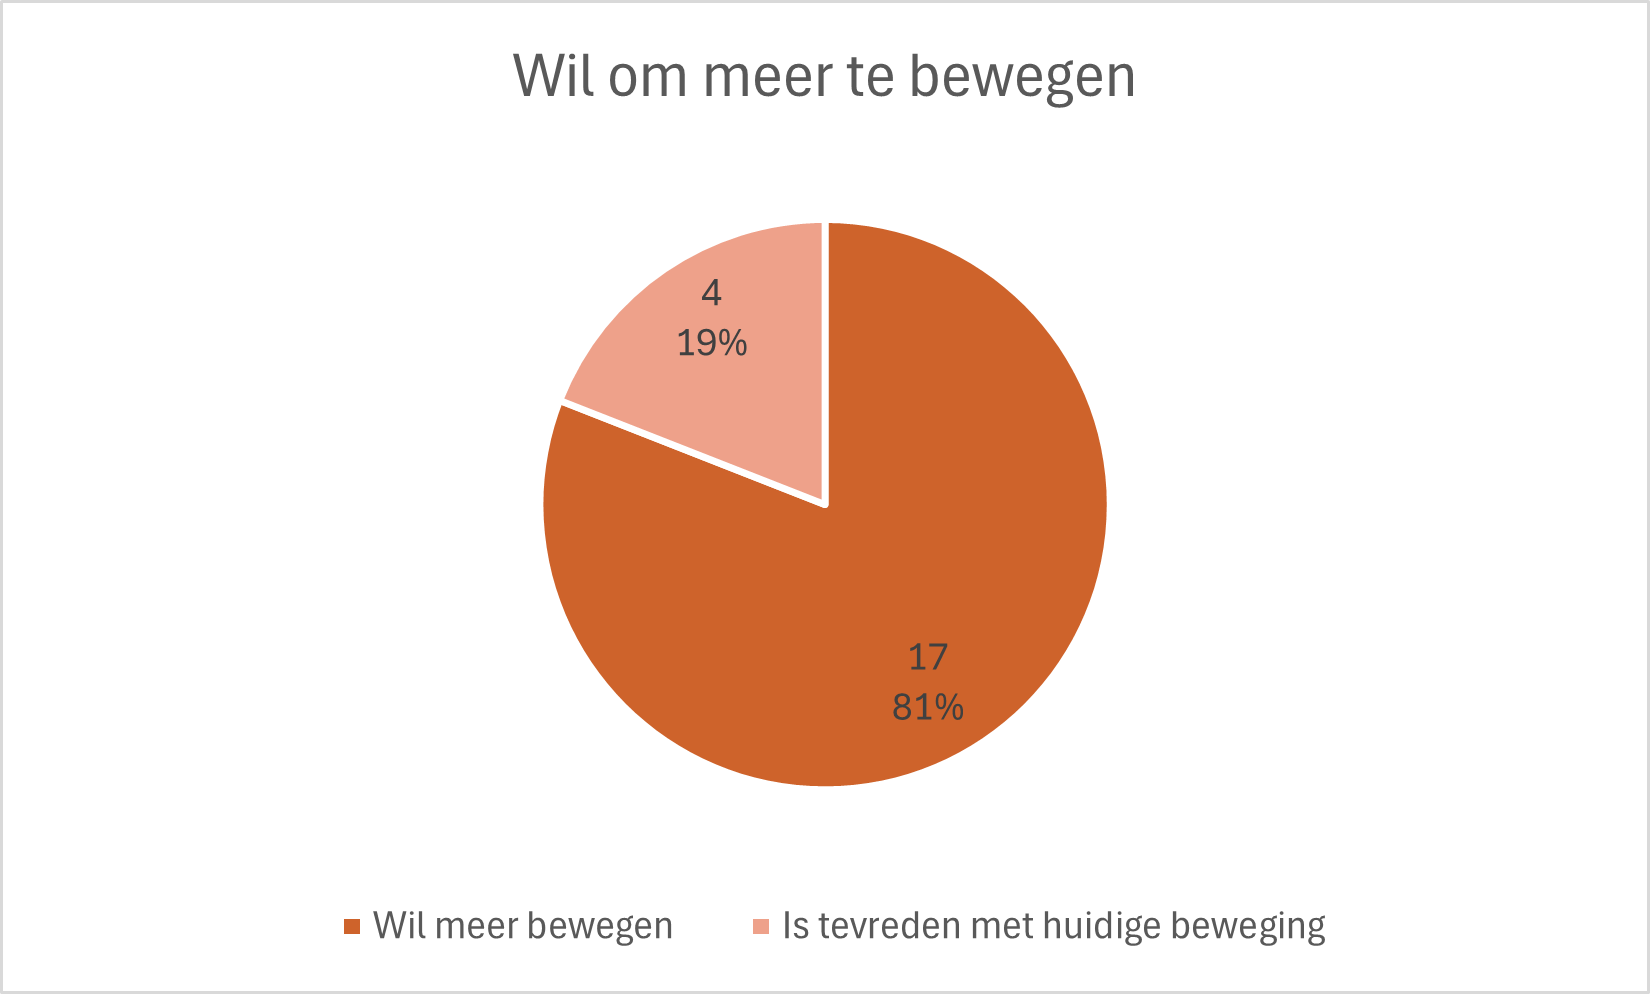
\includegraphics[width=1\textwidth]{MeerSporten}
    \label{fig:meerBewegen}
\end{figure}

Slechts vier van de éénentwintig mensen zijn tevreden met de hoeveelheid sport die ze op dit moment doen. Ruim 81\% is dus niet tevreden en zou liever meer sporten of bewegen (zie figuur \ref{fig:meerBewegen}).

Het grootste probleem voor mensen om meer te sporten, is tijd vinden. Daarnaast staan ook motivatie en wederkerende blessures in de weg. Een minderheid vindt ook geen plezier in het sporten (zie figuur \ref{fig:waarom}).

\begin{figure}[h]
    \caption[Wat houdt u op dit moment tegen om meer te sporten?]{Wat houdt u op dit moment tegen om meer te sporten?}
    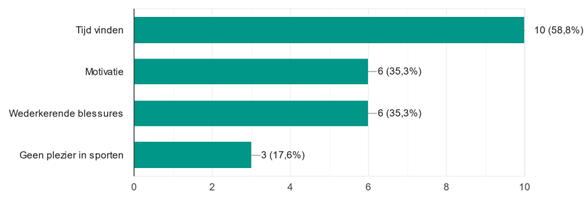
\includegraphics[width=1\textwidth]{Waarom}
    \label{fig:waarom}
\end{figure}

\subsection{Gamification}

Op vlak van het type gamification, is er een duidelijke voorkeur: 76.2\% van de respondenten verkiest een focus op persoonlijke vooruitgang.

Dit kan ook teruggevonden worden in wat belangrijk gevonden wordt in een sportapplicatie. 95.2\% vindt het meten van persoonlijke vooruitgang namelijk belangrijk en 71.4\% vindt ook technische gegevens zien over de activiteit een meerwaarde.

Het valt ook op dat sociale interacties, zoals likes, comments en volgers bijvoorbeeld, net als storend ervaren worden door 47.6\%, dit is tegenstrijdig met de literatuur.

Nog een tegenstrijdigheid die opvalt, is dat 38.1\% uitgedaagd en gemotiveerd wil worden door de applicatie, maar dat 42.9\% het storend vindt meldingen te ontvangen van een sportapplicatie. Dit wil dus zeggen dat deze motivatie op andere manieren dan gewoonlijk opgewekt moet worden.

\section{Sportresultaten}

Evolutie meten. Hoeveel percent haalt de voorgeschreven hoeveelheden.

Niet actieve gebruikers → sporten of gewoon niet ingeven?

\section{Resultaten na gebruik van Move-it!}

Nieuwe vragenlijst maken!

- focus op gevoel
- competitief persoon? -> misschien enkel op competitieve mensen een invloed
- meer sporten in de toekomst?
- wat was anders dan andere sportapplicaties?
    - was dit beter of slechter?
- als u 1 ding zou kunnen veranderen, wat?

%%=============================================================================
%% Conclusie
%%=============================================================================

\chapter{Conclusie}%
\label{ch:conclusie}

OPMERKING: dit hoofdstuk moet ook nog iets beter uitgewerkt worden. U kunt ook hier een skelet terugvinden van zaken die besproken zullen worden.

% TODO: Trek een duidelijke conclusie, in de vorm van een antwoord op de
% onderzoeksvra(a)g(en). Wat was jouw bijdrage aan het onderzoeksdomein en
% hoe biedt dit meerwaarde aan het vakgebied/doelgroep?
% Reflecteer kritisch over het resultaat. In Engelse teksten wordt deze sectie
% ``Discussion'' genoemd. Had je deze uitkomst verwacht? Zijn er zaken die nog
% niet duidelijk zijn?
% Heeft het onderzoek geleid tot nieuwe vragen die uitnodigen tot verder
%onderzoek?

\section{Bespreking van de resultaten}

Uit de eerste vragenlijst kan geconcludeerd worden dat vooral de hoeveelheid dagelijkse beweging met gemiddelde intensiteit niet behaald wordt. Een mogelijke oorzaak van dit resultaat, kan zijn dat mensen die al veel sporten, enkel intensieve activiteiten beschouwen als beweging.

Hier komt nog een conclusie van de waargenomen sportactiviteiten, waarna er teruggekoppeld zal worden naar de literatuurstudie.

Hier zal ook besproken worden of mogelijks de piramide van behoeften (eerder besproken in de literatuurstudie) invloed heeft op het resultaat van dit onderzoek, met andere woorden: werden mensen niet uitgedaagd door het sportplatform doordat er aan de noden in de onderste lagen van de piramide niet voldaan werd.

Antwoord op onderzoeksvraag: ja, een competitief sportplatform kan mensen in een sedentaire job helpen om meer te bewegen, maar enkel als
er voldoende rekening gehouden wordt met hoe gamification geïmplementeerd wordt,
het makkelijk gemaakt wordt op sportgegevens in te geven en er voldoende mensen meedoen die elkaar kennen.

\section{Mogelijkheden tot verder onderzoek}

Zoals eerder besproken, leiden de volgende onduidelijkheden of vragen tot verder onderzoek:

\begin{itemize}
    \item Hoe kan er een onderscheid gemaakt worden tussen intensieve activiteiten en activiteiten met gemiddelde intensiteit?
    \item Geven personen die weinig maar wel intensief sporten enkel deze gegevens in, waardoor het lijkt dat ze minder doen dan mensen die regelmatig een beetje bewegen? Of bewegen ze effectief weinig naast deze intensieve activiteiten?
    \item Welke conclusies kunnen getrokken worden wanneer er een grotere steekproef genomen wordt?
    \item Welk effect heeft een sportplatform met gamification er uit voor mensen die ouder zijn dan de deelnemers van dit onderzoek?
    \item Hoe willen mensen gemotiveerd worden als ze geen meldingen willen ontvangen?
\end{itemize}

%---------- Bijlagen -----------------------------------------------------------

\appendix

\chapter{Onderzoeksvoorstel}

Het onderwerp van deze bachelorproef is gebaseerd op een onderzoeksvoorstel dat vooraf werd beoordeeld door de promotor. Dat voorstel is opgenomen in deze bijlage.

\section*{Samenvatting}

% Kopieer en plak hier de samenvatting (abstract) van je onderzoeksvoorstel.
Beweging speelt een grote rol in zowel de fysieke als de mentale gezondheid van mensen. Bijna één derde van de wereldbevolking beweegt te weinig en ondervindt hier vroeg of laat de nadelen van. Om die reden bespreekt dit onderzoek hoe een sportplatform gebruik kan maken van gamification om medewerkers van \href{https://www.mace-legal.com/}{MACE}, \href{https://www.joule.be/}{Joule} en \href{https://planetb.life/}{PlanetB} aan te zetten om meer te sporten. Bijkomend kan dit er voor zorgen dat de productiviteit positief beïnvloed wordt.

Na een literatuurstudie rond gamification en het belang van beweging, zullen werknemers van eerder genoemde bedrijven geïnterviewd worden om de succescriteria en de benodigdheden van het nieuwe platform te bepalen. Aan de hand van deze criteria zal een platform, in de vorm van een responsive website, gecreëerd worden. Hierin wordt gamification geïmplementeerd en zullen sportgegevens van deelnemende werknemers verzameld en grafisch voorgesteld worden op het platform. Tegelijkertijd zal ook de beleving omtrent het gamification-aspect bevraagd worden. Deze gegevens zullen na een testperiode geanalyseerd worden om te onderzoeken of er een positieve evolutie merkbaar is in de hoeveelheid beweging van de werknemers en of deze ook effectief aan het platform te danken is.

Wanneer rekening gehouden wordt met de sociale aspecten van gamification, geeft de vergaarde kennis momenteel aan dat dit sportplatform wel degelijk een positieve invloed zal hebben op het sportgedrag van de gebruikers. Dit zou op zijn beurt een gunstig effect hebben op de productiviteit van de deelnemende bedrijven.


% Verwijzing naar het bestand met de inhoud van het onderzoeksvoorstel
%---------- Inleiding ---------------------------------------------------------

\section{Introductie}%
\label{sec:introductie}

Een sedentaire job wordt geassocieerd met schadelijke gevolgen voor de algemene gezondheid \autocite{Buckley2015}. Het is dus van groot belang dat voldoende beweging een prioriteit is.

\textcite{Hallal2012} beschouwen 31,1\% van de wereldwijde bevolking als inactief. Dit wil zeggen dat, op het moment van onderzoek, bijna een derde van de volwassen wereldbevolking de vooropgestelde aanbevelingen van ``World Health \linebreak Organization'' (WHO), beschreven door \textcite{Bull2020}, niet haalt. Voor Europa ligt deze waarde zelfs op 34,8\% en zoals op Figuur \ref{fig:inactivity} te zien is, ligt België nog een stuk boven de gemiddelde Europese waarde met 40\% à 49,9\%.

\begin{figure}[t]
    \caption{Fysieke inactiviteit volwassenen (15+) wereldwijd, bij mannen (A) en vrouwen (B) \autocite{Bull2020}}
    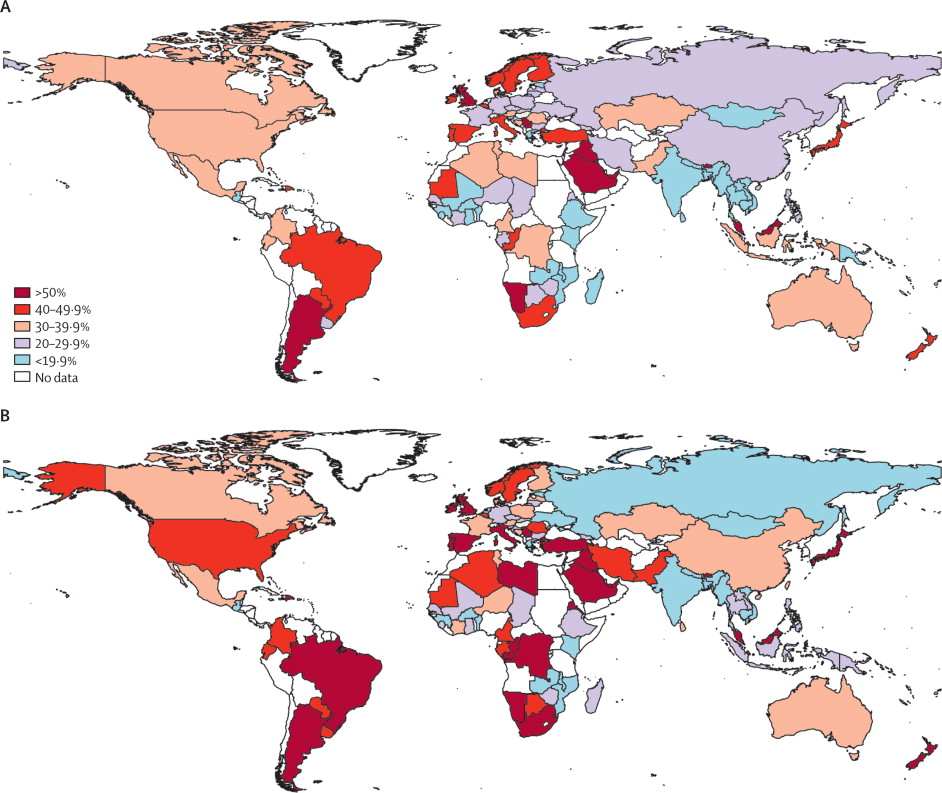
\includegraphics[width=0.5\textwidth]{Inactiviteit}
    \label{fig:inactivity}
\end{figure}

Om deze problematiek te proberen verhelpen, zal een sportplatform ontwikkeld worden. Deze paper onderzoekt hoe gamification hierbij kan helpen. Gamification is in de literatuur beschreven als het gebruiken van spelelementen in een context die niet aan een spel gerelateerd is \autocite{Gaalen2020}.

In de literatuurstudie zal allereerst het belang van voldoende beweging voor een goede gezondheid nog verder gekaderd worden. Daarna zal het effect van die beweging en gezonde levensstijl op productiviteit geïllustreerd worden. Vervolgens zal het concept van gamification diepgaander uiteengezet worden, door onder andere in te zoomen op de meest gebruikte technieken, de sociale en psychologische aspecten en de invloed op het gebruikersgedrag. Ten slotte wordt er gekeken naar bestaande sportapplicaties en -platformen, en beschreven welke vormen van gamification daar in voorkomen.

Nadien zal in de methodologie worden uiteengezet welke stappen er nodig zijn om tot het sportplatform te komen dat, door middel van gamification, werknemers van \textbf{bedrijfX} en \textbf{bedrijfY} motiveert om meer te sporten.

Uiteindelijk kunnen de conclusies van het onderzoek teruggevonden worden.


%---------- Stand van zaken ---------------------------------------------------

\section{Literatuurstudie}%
\label{sec:state-of-the-art}

\subsection{Belang van beweging}

Bij volwassenen wordt een sedentaire levensstijl geassocieerd met schadelijke gevolgen voor de volgende gezondheidskwesties: sterfte in het algemeen, sterfte door hart- en vaatziekten en kanker, het voorkomen van hart- en vaatziekten, diabetes type 2 en kanker \autocite{Bull2020}. Daarnaast gaat verminderde fysieke activiteit ook gepaard met meer depressie-, angst- en stresssymptomen \autocite{Stanton2020}.

Om de kans hierop te verkleinen moeten volwassenen, tussen de 18 en 64 jaar oud, volgens de WHO wekelijks 150 à 300 minuten sporten met gemiddelde intensiteit of 75 à 150 minuten met krachtige intensiteit \autocite{Bull2020}. Voor mensen met een beperking worden dezelfde hoeveelheden sport aangeraden, hoewel daar mogelijks samen met een medisch verantwoordelijke bekeken moet worden in welke mate dit mogelijk is, afhankelijk van de beperking. Voor zwangere of net bevallen vrouwen wordt er minstens 150 minuten per week, met gemiddelde intensiteit, aangeraden.

\subsection{Beweging en productiviteit}

Wanneer de algemene gezondheid van werknemers slecht is, brengt dit kosten mee voor het bedrijf. \textcite{Sjoegaard2016} beschrijven hoe deze kosten gerelateerd zijn aan de mentale en fysieke afwezigheid van werknemers tijdens het werk, met een verminderde productiviteit tot gevolg. Echter, voor personen die sedentair werk uitvoeren en voornamelijk aan een computer werken, zorgt een verhoogde hoeveelheid sport tijdens de vrije tijd voor minder stres en meer energie op de werkvloer \autocite{Hansen2009}. Op die manier leidt het invoeren van regelmatige beweging, door middel van op voorhand opgestelde oefeningen en een zorgvuldige begeleiding, volgens \textcite{Cancelliere2011} tot een positief effect op de productiviteit. In die mate dat \textcite{Sjoegaard2016} stellen dat dit effect de eventuele uitgaven in verband met sportactiviteiten overstijgen.

\subsection{Gamification}

Volgens \textcite{Deterding2011} is gamification te beschrijven als het gebruiken van speldesignelementen in een niet-spelgerelateerde context. Gamification bestaat uit drie hoofdonderdelen: de gebruikte techniek, de psychologische uitkomsten en de verdere invloed op het gedrag \autocite{Hamari2014}. Daarnaast zijn sociale aspecten ook essentieel: door het ontstaan van een competitie streven mensen ernaar erkenning te ontvangen \autocite{Hamari2013}.

\subsubsection{Meest gebruikte technieken}

\textcite{Hamari2014} somt punten, scoreborden en vooropgestelde uitdagingen op als de drie \linebreak meest voorkomende technieken. Daarnaast komen ook volgende methodes veelvuldig voor: het gebruik van levels, en eventueel een daarbij horend verhaal, beloningen, een overzicht van vooruitgang of het bekomen van badges, die bijvoorbeeld de beste gebruiker in een bepaalde categorie aanduiden \autocite{Dong2012,Flatla2011,Li2012}.
Daarbij kunnen de gehanteerde technieken verder ingevuld worden naar wens. Zo kunnen beloningen bijvoorbeeld bestaan uit, maar daarom niet gelimiteerd worden tot, een donatie aan een gekozen goed doel of een eervolle vermelding op een intern bedrijfsevenement.

\subsubsection{Sociale aspecten}

Er zijn twee belangrijke sociale aspecten om in acht te nemen wanneer gamification geïmplementeerd wordt.

Enerzijds is er erkenning, wat beschreven kan worden als de sociale feedback die gebruikers krijgen op hun gedrag \autocite{Cheung2011}.
Wanneer een dienst, zoals het aanbieden van een platform met gamification, erkenning van de andere gebruikers oplevert, wordt die dienst positiever ervaren \autocite{Preece2001}.
\textcite{Hamari2013} suggereren dat er vervolgens, als gevolg van de ontvangen erkenning, een bepaalde bereidheid ontstaat om de erkenning wederkerig te maken. Hierdoor zal de tegenpartij ook op zijn beurt de dienst positiever ervaren.

Anderzijds is er sociale invloed, wat verwijst naar de perceptie van een individu over het belang dat anderen hechten aan een bepaald doelgedrag en of ze verwachten dat iemand dat gedrag zal vertonen \autocite{Ajzen1991}. Specifiek voor een platform dat gamification implementeert, kan er sociale invloed ontstaan door het zien van wat andere gebruikers op het platform presteren. Hierdoor wordt namelijk een verwachtingspatroon gecreëerd en zetten gebruikers elkaar aan tot het behalen van een bepaald doelgedrag, zoals vaker sporten.

\subsubsection{Psychologische aspecten}

Wanneer psychologische gevolgen op de gebruiker bevraagd zijn, wordt er vooral gefocust op motivatie, attitude en plezier \autocite{Hamari2014}. \textcite{Cheong2013} werkte een online quiz uit die gamification gebruikt, met als doel om bijleren te motiveren en leuker te maken. Uit een bevraging  na de quiz bleek dat 40,79\% van de deelnemers enthousiast en 46,05\% van de deelnemers tevreden was tijdens de quiz. Daarenboven was het merendeel (77,63\%) van de deelnemers voldoende gemotiveerd om de quiz te vervolledigen.

\subsubsection{Invloed op gedrag}

\textcite{Kari2016} stellen dat gamification in sportapplicaties een positieve invloed heeft op de intrinsieke bewegingsmotivatie, wat ervoor zorgt dat gebruikers gaan handelen naar een bepaald doelgedrag. \textcite{PoloPena2020} bevestigen dit, maar voegen hier wel aan toe dat gamification een grotere invloed heeft op vrouwen dan op mannen, en op oudere mensen dan op jongere gebruikers.

Studies van \textcite{Hamari2013a} hebben aangetoond dat de resultaten van gamification mogelijks niet voor alle gebruikers op lange termijn doeltreffend zijn, en de invoering ervan mogelijks niet op iedereen het gewenste effect heeft.
Anderzijds zal het verwijderen van spelelementen uit een dienst schadelijke gevolgen voor de gebruikers hebben die wel nog betrokken zijn tot het gamification-aspect: zo kan een gebruiker plots al diens vooruitgang of verdiende badges verliezen.

\subsection{Bestaande sportapplicaties}

Hieronder volgt een diverse greep uit de bestaande mobiele en desktop sportapplicaties en -platformen en welke spelelementen daarin gebruikt worden.

\href{https://www.strava.com/}{Strava} is een applicatie waarmee gebruikers hun sportprestaties kunnen bijhouden. \textcite{Barratt2017} stelt dat deze applicatie gamification toepast, zoals uitdagingen en persoonlijke en trainingsvooruitgang.

\href{https://www.nike.com/be/en/nrc-app}{Nike Run Club} is een loopapplicatie met meer dan 10 miljoen downloads\footnote{\href{https://bootcamp.uxdesign.cc/how-the-nike-run-club-app-got-runners-hooked-2850c7654fc5}{How the Run Club App got runners hooked - Leevey}} op de Google Play Store en de App Store. Deze applicatie maakt het mogelijk voor lopers om een looptraining vast te leggen, punten te verdienen en andere gebruikers uit te dagen. Daarnaast kunnen ze eigen doelstellingen aanmaken en delen, zodat samen naar een gezamenlijk doel gewerkt kan worden \autocite{StaalnackeLarsson2013}.

Een derde voorbeeld is \href{https://connect.garmin.com/}{Garmin Connect}. Het verschil met de vorige twee applicaties is dat dit platform enkel voor gebruikers met een Garmin-toestel bedoeld is. Deze applicatie focust vooral op badges \autocite{Ilhan2019}. Het behalen van zulke badge kan dan punten opleveren en de mogelijkheid geven tot het behalen van nieuwe, meer uitdagende badges. Om negatieve gevoelens van frustratie op een mindere dag tegen te gaan, krijgt de gebruiker de optie om andere, niet fysieke activiteiten uit te voeren om ook dan punten te verdienen.

Een platform dat aan de criteria van deze casus voldoet, bestaat nog niet en zal dus ontwikkeld moeten worden in een volgende fase van het onderzoek.


%---------- Methodologie ------------------------------------------------------
\section{Methodologie}
\label{sec:methodologie}

Het onderzoek zal beginnen met een literatuurstudie die het belang van voldoende beweging kadert, vervolgens bespreekt wat het effect hiervan is op productiviteit en tenslotte gamification verder uitdiept. Het is bij dit laatstse belangrijk om technieken te identificeren die van toepassing zijn op deze specifieke casus. De resultaten hiervan kunnen gebruikt worden in de volgende fase.

Deze volgende fase bestaat uit een bevraging bij IT-werknemers van \textbf{bedrijfX} en \textbf{bedrijfY}. De bedoeling hiervan is enerzijds achterhalen in \linebreak welke mate sport en beweging een rol speelt in hun dagelijkse leven op het moment van het interview, en anderzijds te weten komen in welke mate en op welke manieren deze werknemers gestimuleerd kunnen worden om meer te gaan sporten, aan de hand van een competitief sportplatform. Hier kan ook de theorie die verkregen is uit de literatuurstudie getoetst worden.

Steunend op de bekomen resultaten uit zowel de literatuurstudie als de analyse van de gebruikersinterviews, zal dan een applicatie ontwikkeld worden. Het platform zal bestaan in de vorm van een responsive website, waarin sportgegevens van deelnemende werknemers worden verzameld aan de hand van applicaties en hun ''Application Programming Interface'' (API) zoals \linebreak \href{https://developers.strava.com/}{Strava}, \href{https://dev.fitbit.com/}{Fitbit} en \href{https://developer.garmin.com/gc-developer-program/overview/}{Garmin Connect}. Deze gegevens zullen in combinatie met gamification gebruikt worden om een competitie tussen de deelnemende bedrijven op te zetten.

Deze POC zal dan dienen om de hypotheses te toetsen: heeft het competitief sportplatform, dat gebruik maakt van gamification, een positieve invloed op het sportgedrag van werknemers in een sedentaire job? Om deze vraag te beantwoorden zullen opnieuw gebruikersinterviews plaatsvinden, met dezelfde personen die voor aanvang van de ontwikkelingsfase geïnterviewd zijn en die voor een periode van enkele weken deze POC hebben kunnen gebruiken. Een grondige analyse van de sportgegevens op het platform en de antwoorden van deze ondervraging, leiden tot de conclusie van dit onderzoek.


%---------- Verwachte resultaten ----------------------------------------------
\section{Verwacht resultaat}%
\label{sec:verwachte_resultaten}

De verworven kennis geeft momenteel aan dat een sportplatform met implementatie van gamification wel degelijk een positieve invloed zal hebben op het sportgedrag van gebruikers. Het verwachtte resultaat gaat er van uit dat er voldoende aandacht besteed wordt aan het sociale aspect van gamification en dat de gebruikers ook hun persoonlijke ontwikkeling en groei kunnen opmerken op het platform.

Ten gevolge van de positieve invloed op het sportgedrag van de deelnemende bedrijven, \linebreak wordt ook minder stress en een verbeterde productiviteit en tevredenheid op de werkvloer verwacht.

%%---------- Andere bijlagen --------------------------------------------------
% TODO: Voeg hier eventuele andere bijlagen toe. Bv. als je deze BP voor de
% tweede keer indient, een overzicht van de verbeteringen t.o.v. het origineel.
%\input{...}

%%---------- Backmatter, referentielijst ---------------------------------------

\backmatter{}

\setlength\bibitemsep{2pt} %% Add Some space between the bibliograpy entries
\printbibliography[heading=bibintoc]

\end{document}
